\documentclass[10pt]{beamer}

\usetheme[progressbar=frametitle]{metropolis}
\usepackage{appendixnumberbeamer}

\usepackage{booktabs}
\usepackage[scale=2]{ccicons}

\usepackage{pgfplots}
\usepgfplotslibrary{dateplot}

\usepackage{xspace}
\newcommand{\themename}{\textbf{\textsc{metropolis}}\xspace}

\title{A Study of Charm Quark Correlations}
\subtitle{PHY 371C: Presentation}
\date{\today}
\date{}
\author{Dev Desai}
% \titlegraphic{\hfill\includegraphics[height=1.5cm]{logo.pdf}}

\begin{document}

\maketitle

\begin{frame}{Table of contents}
  \setbeamertemplate{section in toc}[sections numbered]
  \tableofcontents[hideallsubsections]
\end{frame}

\section[Introduction]{Introduction}

\subsection{Motivation}

\begin{frame}[fragile]{Motivation}
Why study charm hadrons?

    \begin{itemize}
        \item Charm quarks are created almost exclusively in the initial hard scattering 
        \item Allows us to probe QCD collision dynamics.
    \end{itemize}
\end{frame}

\subsection{Research Question}

\begin{frame}[fragile]{Research Question}
\textbf{How do the kinematic distributions of charm hadrons produced in high-energy collisions reflect the underlying charm production mechanisms?}
\end{frame}

\subsection{Goals}

\begin{frame}{Goals}
\begin{itemize}
    \item Read and learn the basics of particle physics.
    \item Familiarize myself with Monte Carlo event generators like Pythia, and understand their limitations
    \item Explore the various factors affecting collisions, such as eCM, pT Hard, and particle filtering, and analyze their effects on charm quark production and kinematic properties
    \item Develop a strong foundation and passion for particle physics data analysis and theory
    \item Publish a GitHub repo to accelerate future undergraduate research
\end{itemize}
\end{frame}

\section{Theory Background}

\begin{frame}{Hard Scattering and Hadronization}

\textbf{Hard Scattering:}
\begin{itemize}
    \item High-energy parton-parton collisions (e.g., \( gg \to c\bar{c} \))
    \item Sets the initial kinematic scale of the event
\end{itemize}

\textbf{Hadronization:}
\begin{itemize}
    \item Partons (quarks, gluons) cannot exist freely
    \item They transform into hadrons (e.g., \( c \to D^0 \), \( \Lambda_c \))
\end{itemize}

\end{frame}

\begin{frame}{Transverse Momentum (\( p_T \))}

\[
p_T = \sqrt{p_x^2 + p_y^2}
\]

\begin{itemize}
    \item Momentum in the plane \textbf{perpendicular} to the beam
    \item Collisions at the LHC happen along the z-axis — \( p_T \) is what we actually measure
    \item High \( p_T \) implies a more energetic process
\end{itemize}

\end{frame}

\begin{frame}{Azimuthal Angle (\( \phi \))}

\begin{itemize}
    \item Angle in the transverse (x-y) plane
    \item Ranges from \( -\pi \) to \( \pi \)
    \item Used in angular correlations (e.g., \( \Delta\phi \) between hadrons)
    \item Distribution is usually flat → no preferred direction
\end{itemize}

\end{frame}

\begin{frame}{Rapidity (\( y \))}

\[
y = \frac{1}{2} \ln\left(\frac{E + p_z}{E - p_z}\right)
\]

\begin{itemize}
    \item Measures how forward or backward a particle goes
    \item Useful for massive particles (like charm hadrons)
    \item Boost-invariant along z-axis — great for comparing frames
\end{itemize}

\end{frame}

\begin{frame}{Pseudorapidity (\( \eta \))}

\[
\eta = -\ln\left[\tan\left(\frac{\theta}{2}\right)\right]
\]

\begin{itemize}
    \item Approximation of rapidity for \textbf{massless or high-energy} particles
    \item Defined purely by the angle \( \theta \) from the beamline
    \item Detectors use \( \eta \) because they measure angle, not energy directly
\end{itemize}

\end{frame}

\begin{frame}{Why Use \( \eta \) and \( y \), Not \( \theta \)?}

\begin{itemize}
    \item Detectors are cylindrical, aligned along the beam (z-axis)
    \item Measuring the polar angle \( \theta \) precisely is hard
    \item \( \eta \) and \( y \) are designed to work well with the detector geometry and boost invariance
\end{itemize}

\end{frame}

\section{Pythia}

\begin{frame}{What is Pythia?}
\textbf{Pythia} is a Monte Carlo event generator used to simulate high-energy particle collisions, especially in proton-proton environments like those at the LHC.

\vspace{0.5em}
\begin{itemize}
    \item Models the full evolution of an event:
    \begin{itemize}
        \item \textbf{Hard scattering}: primary parton interaction (e.g., charm quark production).
        \item \textbf{Parton showering}: emission of gluons and quarks (initial/final state radiation).
        \item \textbf{Hadronization}: transition of partons into observable hadrons.
        \item \textbf{Decay}: of unstable hadrons into final-state particles.
    \end{itemize}
    \item Highly configurable: allows tuning of energy, cuts (like \texttt{pTHatMin}), and filtering for specific processes or particles.
\end{itemize}
\vspace{0.5em}
\textit{Used extensively in both theory and experimental workflows to simulate detector-level events and explore particle production dynamics.}
\end{frame}

\begin{frame}{Pythia as a Tool}
How do we specifically need to use Pythia?
\begin{itemize}
    \item We wish to study charm quarks, which are sparsely produced.
    \item We then need to analyze many events to gain a useful amount of data
    \item Pythia is a simulator, but we don't want to run simulations each time we do an analysis
    \item $\rightarrow$ Need a data structure which stores all event info, including kinematics, production vertex, and mother daughter relations
\end{itemize}
\end{frame}

\begin{frame}{Data Structure for Storing Events}
\textbf{Three possibilities}
\begin{enumerate}
    \item Find a built in Pythia command, reminiscent of Ali-physics analysis
    \item Use hepMC, a general high energy physics data structure, which is consistent throughout all event generators
    \item Build our own data structure
\end{enumerate}
\vspace{1em}
I experimented with both Python and C++ scripts and documentation for each option
\end{frame}

\begin{frame}{What didn't work}
\textbf{1. No built in commands available through Pythia}

\vspace{1em}
\textbf{2. hepMC}
\begin{itemize}
    \item Various file formats available, such as default ASCII, binary, ROOT, and ROOT trees
    \item hepMC also has built in parsing methods to make analysis easy
    \begin{itemize}
        \item ASCII (Python \& C++), works, but incredible large file size.
        \item Binary (only C++)
        \item ROOT and ROOT Trees (only C++), ran into many dependency issues
    \end{itemize}
    \item Overall, hepMC could work, but is difficult to set up and requires C++ if we want to store a significant number of events
\end{itemize}
    
\end{frame}

\begin{frame}{What did work}

Created my own data structure: created custom ROOT tree, which branched on TParticle (ROOT class which stores particle information).

\textbf{  } 

\textbf{Benefits}
\begin{itemize}
    \item Entirely based on Python
    \item Easy setup with Conda environments
    \item Uses TParticle, which makes for easy querying of the data structure for any kinematics or decay chain information you may need
    \item Compact file size: \textasciitilde20\text{\%} the size of hepMC ASCII format
\end{itemize}
\end{frame}

\begin{frame}{Limitations of Pythia}

As I was testing the various data structures, I wanted to ensure that each was storing the same information.

\textbf{Two tests:} PDG (particle identifier) counts, and pion mothers' PDG counts.
\begin{itemize}
    \item Found unphysical artifacts (PDG of 90, which isn't a particle) which are likely intermediate internal Pythia objects in my data structure.
    \item Found an extremely high number of gluons (PDG of 21) in the hepMC ASCII
    \item Inconsistent, but similar number of each type of quarks between the two
\end{itemize}
\end{frame}

\begin{frame}{Limitations of Pythia}

\textbf{What was the reason for these discrepancies?}

$\rightarrow$ Pythia is \textit{not} accurate to the quark/gluon level. 
\vspace{1em}

\textbf{Solution?}

$\rightarrow$ Filter out all quarks and gluons during analysis
\vspace{1em}

\textit{When I ran both tests with this filtering, there weren't any more discrepancies. Yay! We can now move onto physics. Oh, and by the way, I am analyzing proton-proton collisions}
    
\end{frame}

\section{Phase Space Cut Analysis}

\begin{frame}{Default Charm Production Frequency}

We wish to analyze charmed hadrons to understand charm production mechanisms. Hence we need a sizeable dataset of charm quarks.

But, if we run default Pythia events, only 3.3\text{\%} of events have charm quarks. 

$\rightarrow$ Most of our data set is unusable to us. 

$\rightarrow$ Inefficient simulation and analysis
    
\end{frame}

\begin{frame}{Default Charm Production Frequency}

\begin{figure}[h]
  \centering
  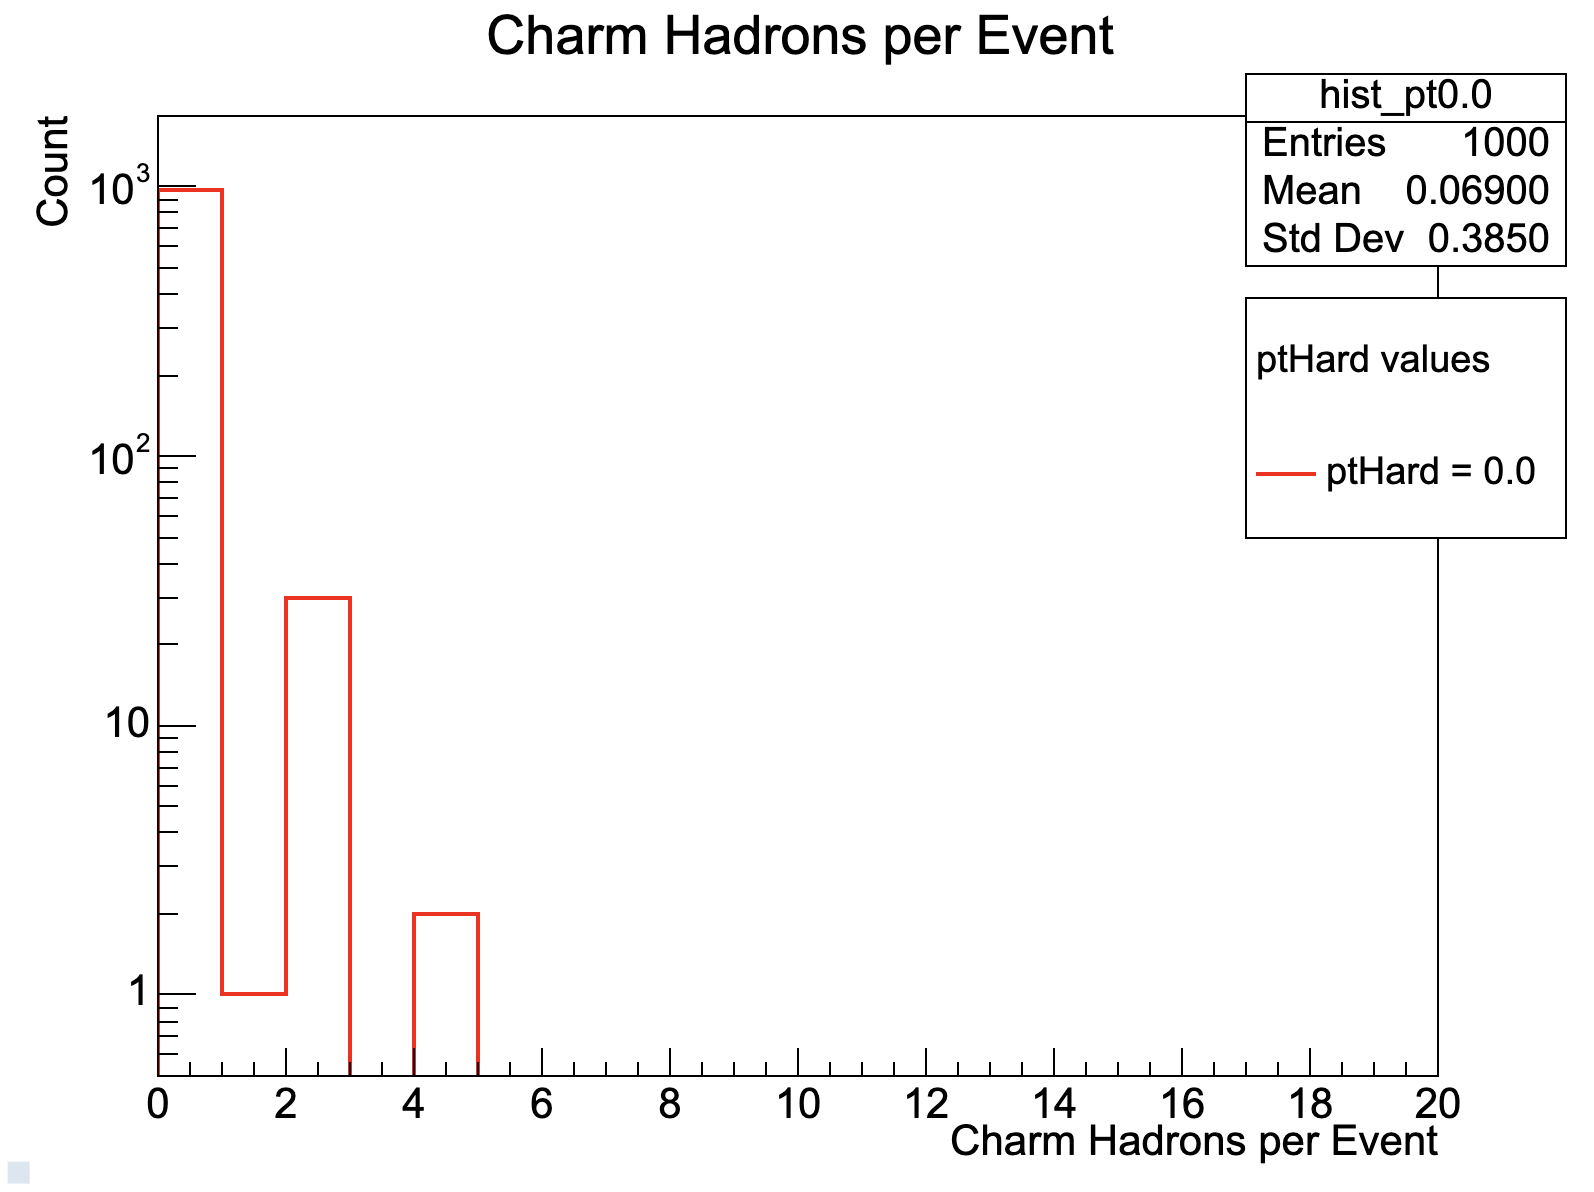
\includegraphics[width=0.9\linewidth]{pt0.png}
  \caption{Histogram of charm production frequency}
  \label{fig:pt0}
\end{figure}
\end{frame}

\begin{frame}{pTHatMin}

\textbf{How can we get a dataset which contains more charmed hadrons?}
\begin{itemize}
    \item Charmed hadrons, because of their higher mass and energy, are produced in more energetic hard scattering events. 
    \item We can quantify with pT Hard - how much transverse momentum is in the scattering event
    \item We can implement \textit{phase space cuts} (using pTHatMin) - as Pythia is generating an event, if the pTHard is not > pTHatMin, it rejects the event and doesn't store it
\end{itemize}
\end{frame}

\begin{frame}{pTHatMin Analysis}

\begin{figure}
    \centering
    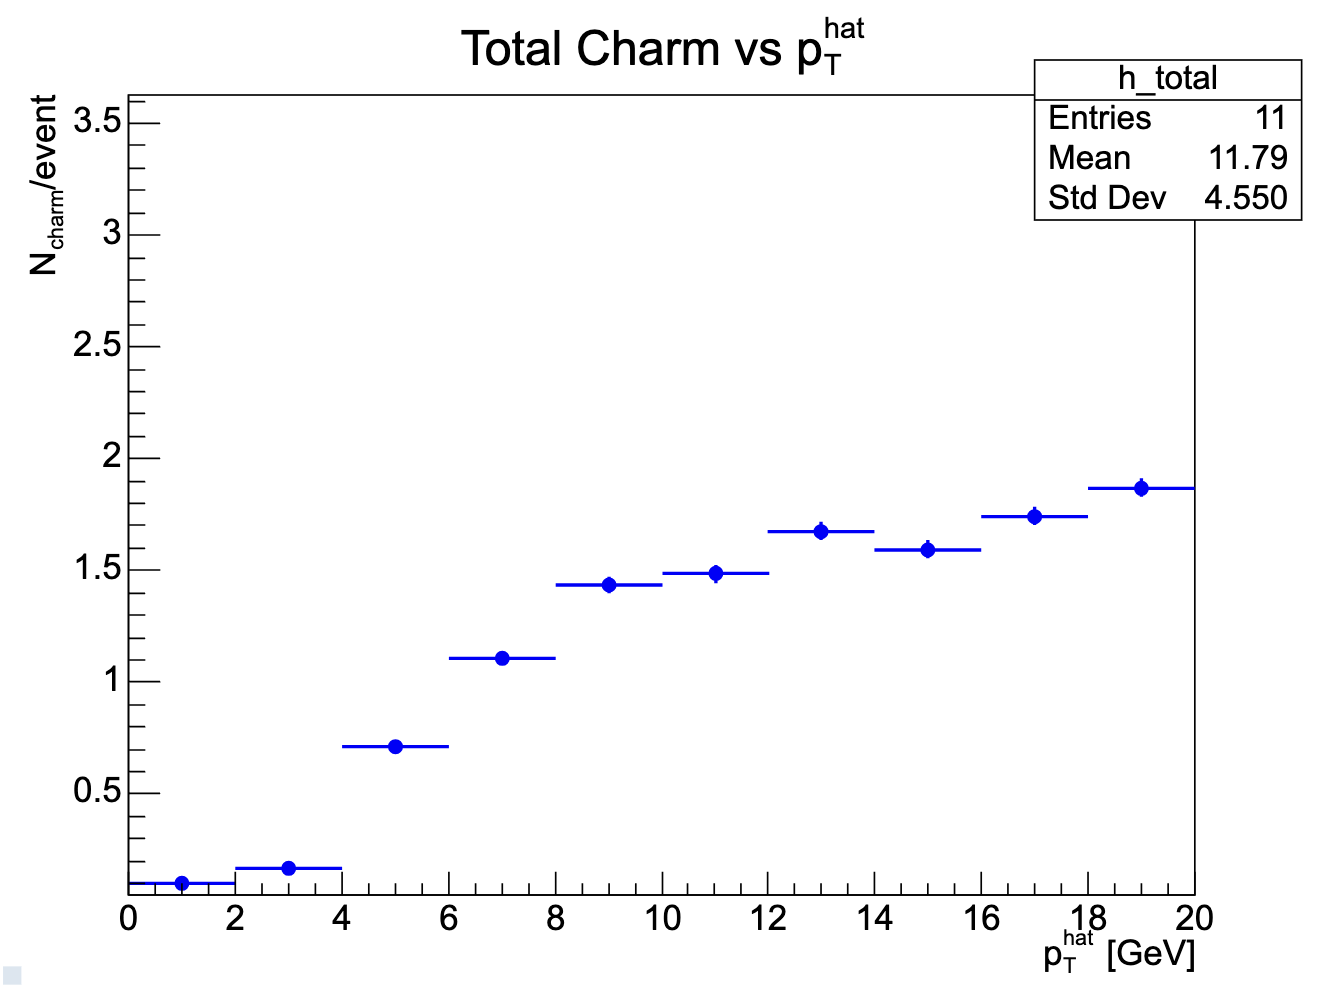
\includegraphics[width=0.8\linewidth]{ptsummary.png}
    \caption{Phase space cuts' relation to charm production. \textbf{Note:} after pTHatMin = 10, starts to plateau}
    \label{fig:ptsummary}
\end{figure}
    
\end{frame}

\begin{frame}{pTHatMin Analysis}

\begin{figure}
    \centering
    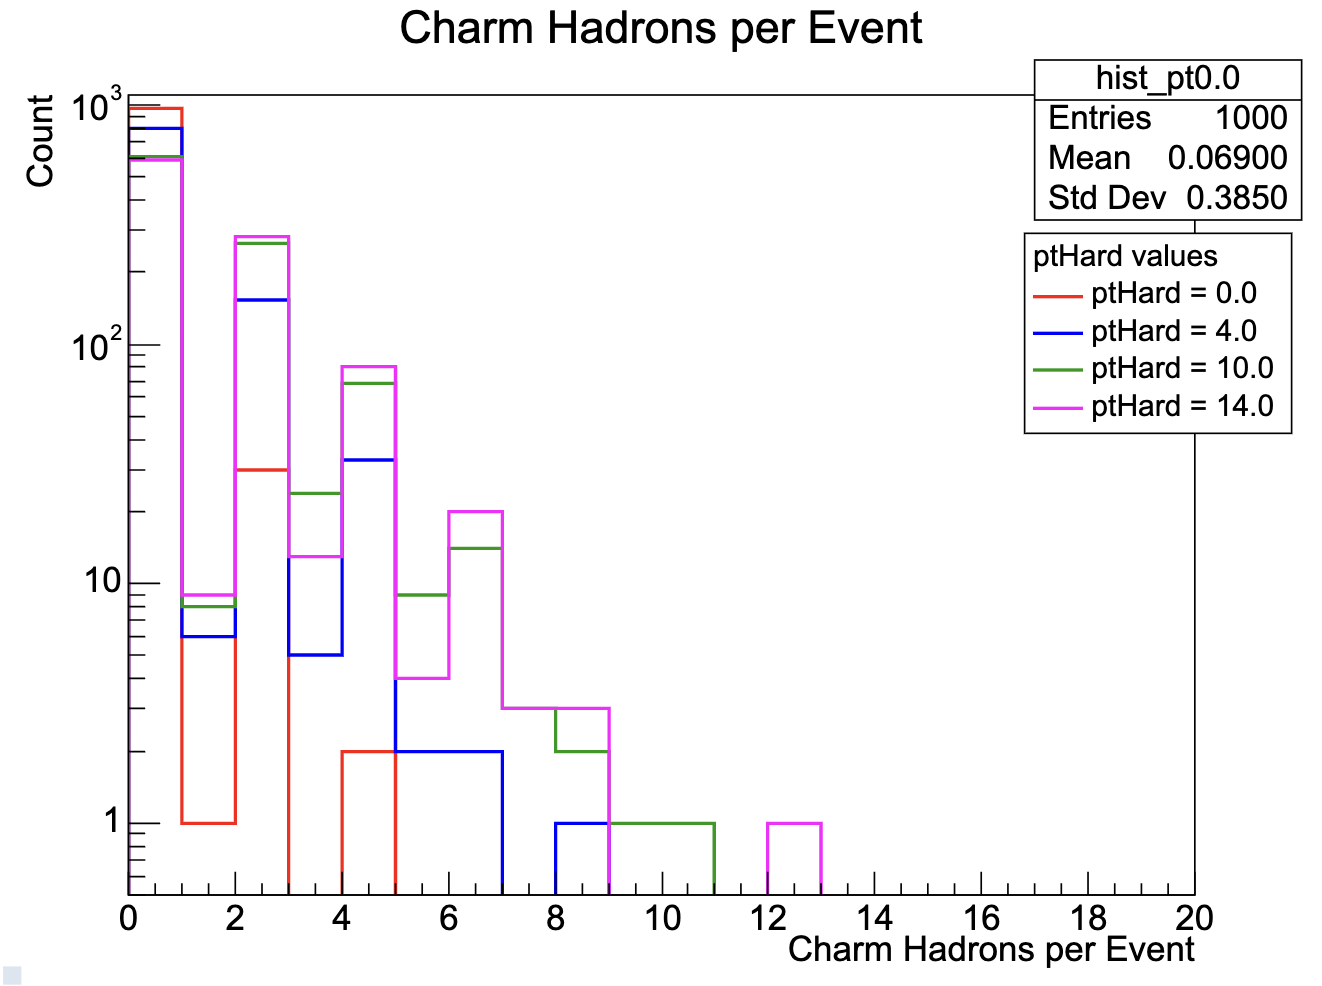
\includegraphics[width=0.8\linewidth]{charmperevent.png}
    \caption{More context behind pTHatMin vs charm hadron production.}
    \label{fig:ptcharmperevent}
\end{figure}
    
\end{frame}

\begin{frame}{pTHatMin Analysis}

\begin{figure}
    \centering
    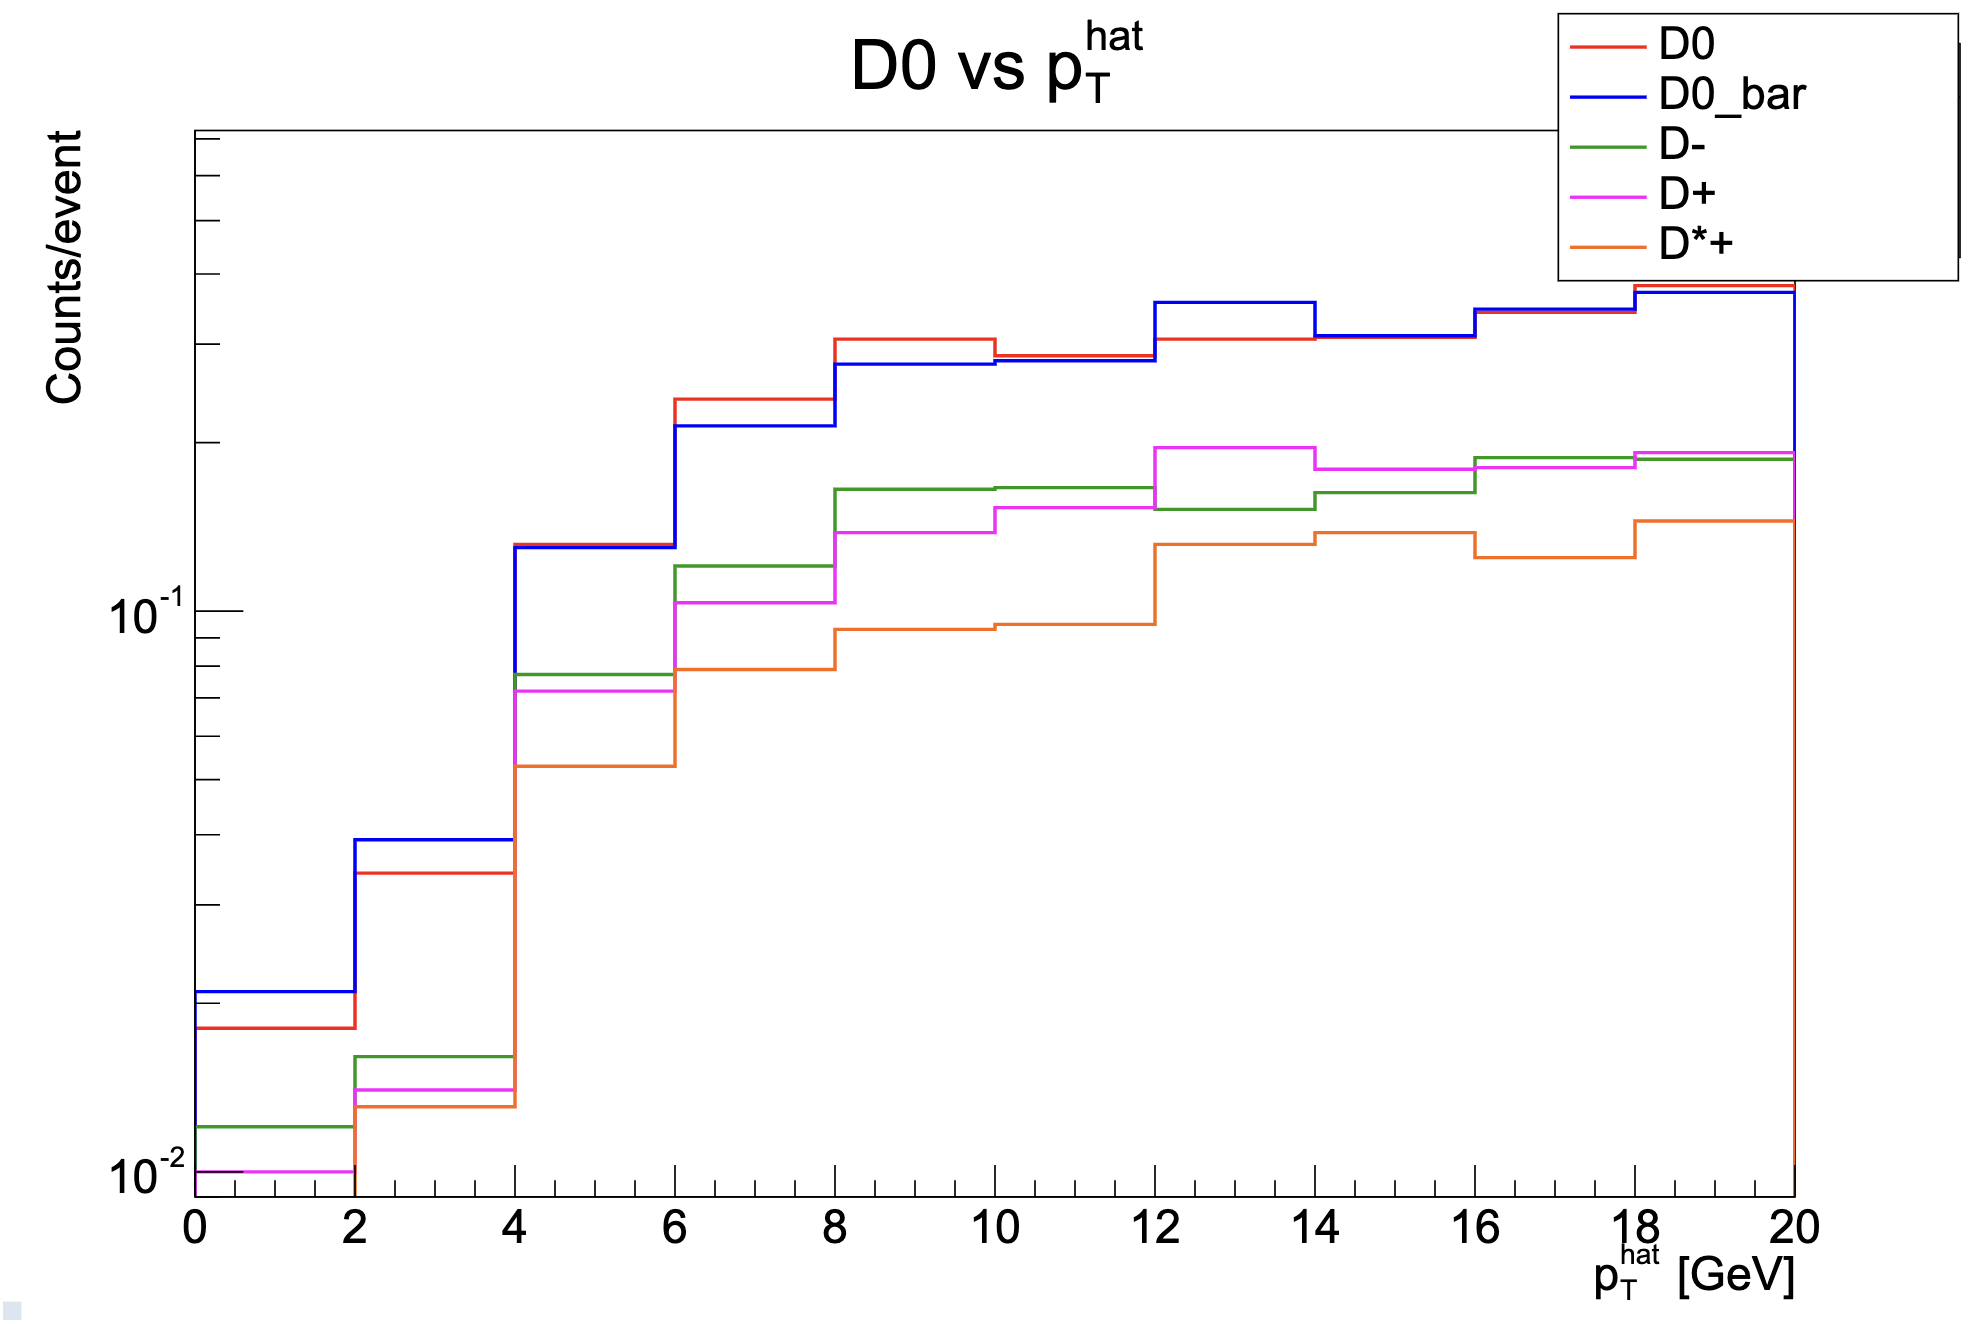
\includegraphics[width=0.85\linewidth]{ptD.png}
    \caption{D Meson production with respect to pThatMin. \textbf{Note:} D0 meson's are produced at higher rates than other D mesons}
    \label{fig:ptsummary}
\end{figure}
    
\end{frame}

\begin{frame}{pTHatMin Summary}

\begin{itemize}
    \item As we increase pTHatMin, Pythia simulations take much longer, as it is rejecting more and more events because they do not meet the pT Hard cut. 

    \item \textbf{I chose to use pTHatMin = 10 GeV for all future work}, as there was not any considerable gains after.
\end{itemize}

$\rightarrow$ Next, I simulated 10,000 events, which took a couple of minutes, but for future work, 1 million events is preferable. This will take a significant time to simulate, and the diminishing charm production gains after pTHatMin of 10 GeV might be not worth the extra time when running the simulation.
    
\end{frame}


%%%%%%%%%%%%
\section{Charm Multiplicity Analysis}

\begin{frame}{Charmed Hadron Count}

\begin{figure}
    \centering
    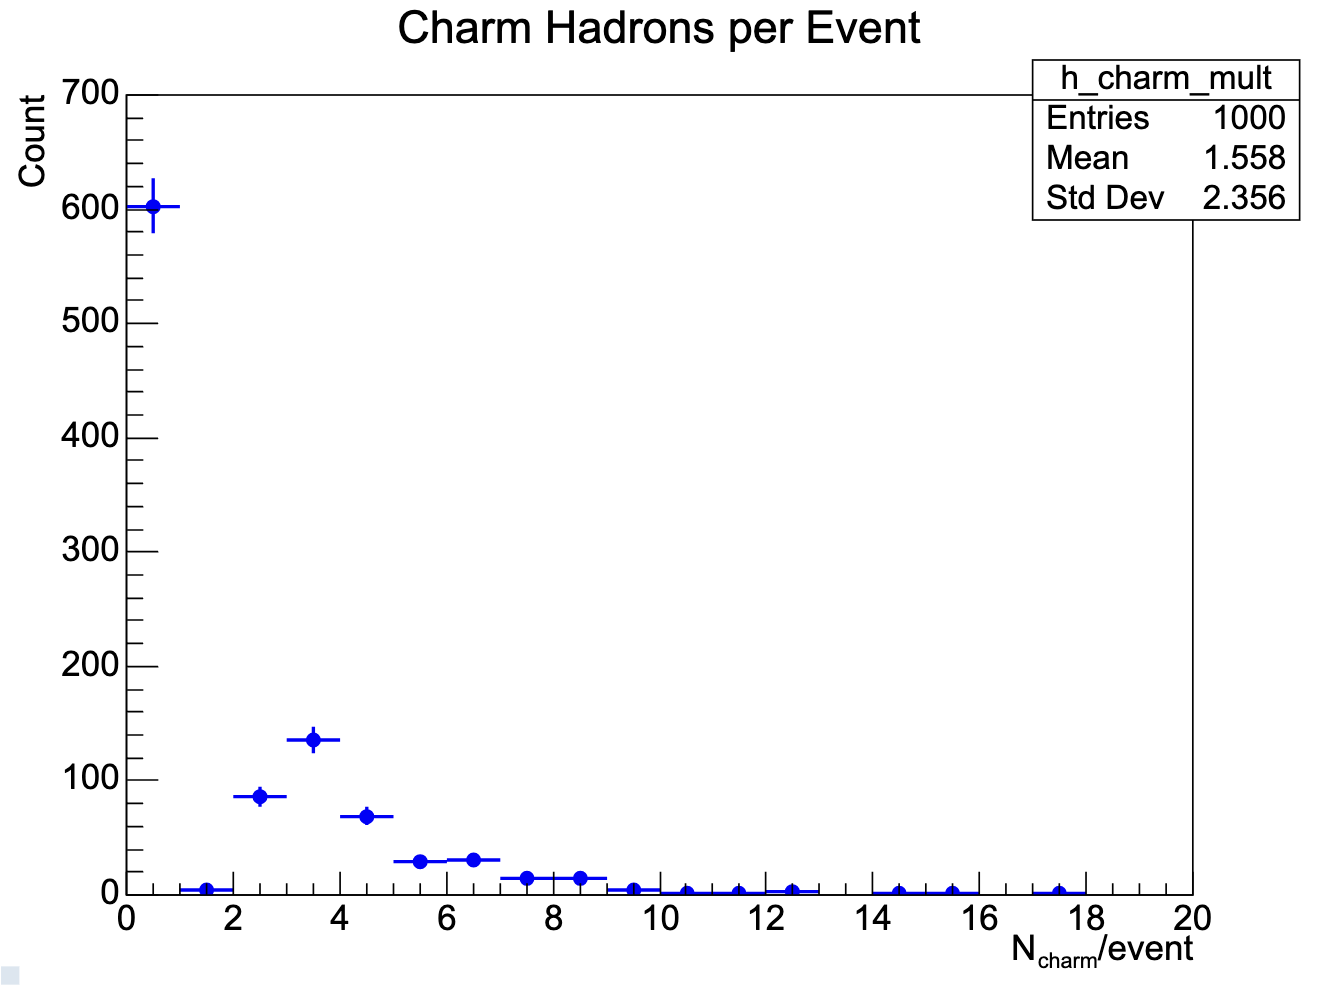
\includegraphics[width=0.6\linewidth]{mult1.png}
    \caption{A histogram of charmed hadron production per event}
    \label{fig:mult1}
\end{figure}

We see something odd here: charm quarks, and thereby hadrons, are most commonly produced in pairs. But, we see that there are more events with 3 charm hadrons than 2!
    
\end{frame}

\begin{frame}{Charm Production Processes}

\textbf{Pair Production}: $gg \rightarrow cc$ or $qq \rightarrow cc$
\begin{itemize}
    \item Produces a pair charm quarks $\rightarrow$ 2 charm hadrons (leading to even count)
    \item Is the most common production mechanism
\end{itemize}

\textbf{Flavor Excitation:} $gc \rightarrow gc$ or $qc \rightarrow qc$
\begin{itemize}
    \item Produces 1 charm quark $\rightarrow$ 1 charm hadron (leading to odd count)
    \item Rarely happens
\end{itemize}

\textbf{Gluon Splitting:} $g \rightarrow cc$
\begin{itemize}
    \item Produces a pair charm quarks $\rightarrow$ 2 charm hadrons (leading to even count)
\end{itemize}

\end{frame}

\begin{frame}{Charm Production Processes}

Charm hadrons are most commonly formed in pairs, so why the peak at 3 per event? 
\begin{itemize}
    \item When $D*$ mesons are produced, they then decay into a D meson. So, by counting all charmed hadrons, including higher energy states such as D*, we are \textit{double counting}.

    \item To alleviate this, instead of filtering for all charmed hadrons, we can filter for "final" charm hadrons, where they won't decay into another charm hadron. 

    \item These include $D0,\overline{D0}, D+, D-, Ds+, Ds-, \Lambda c+, \Lambda c-$

\end{itemize}
\end{frame}

\begin{frame}{Accounting for D* Decay}

\begin{figure}
    \centering
    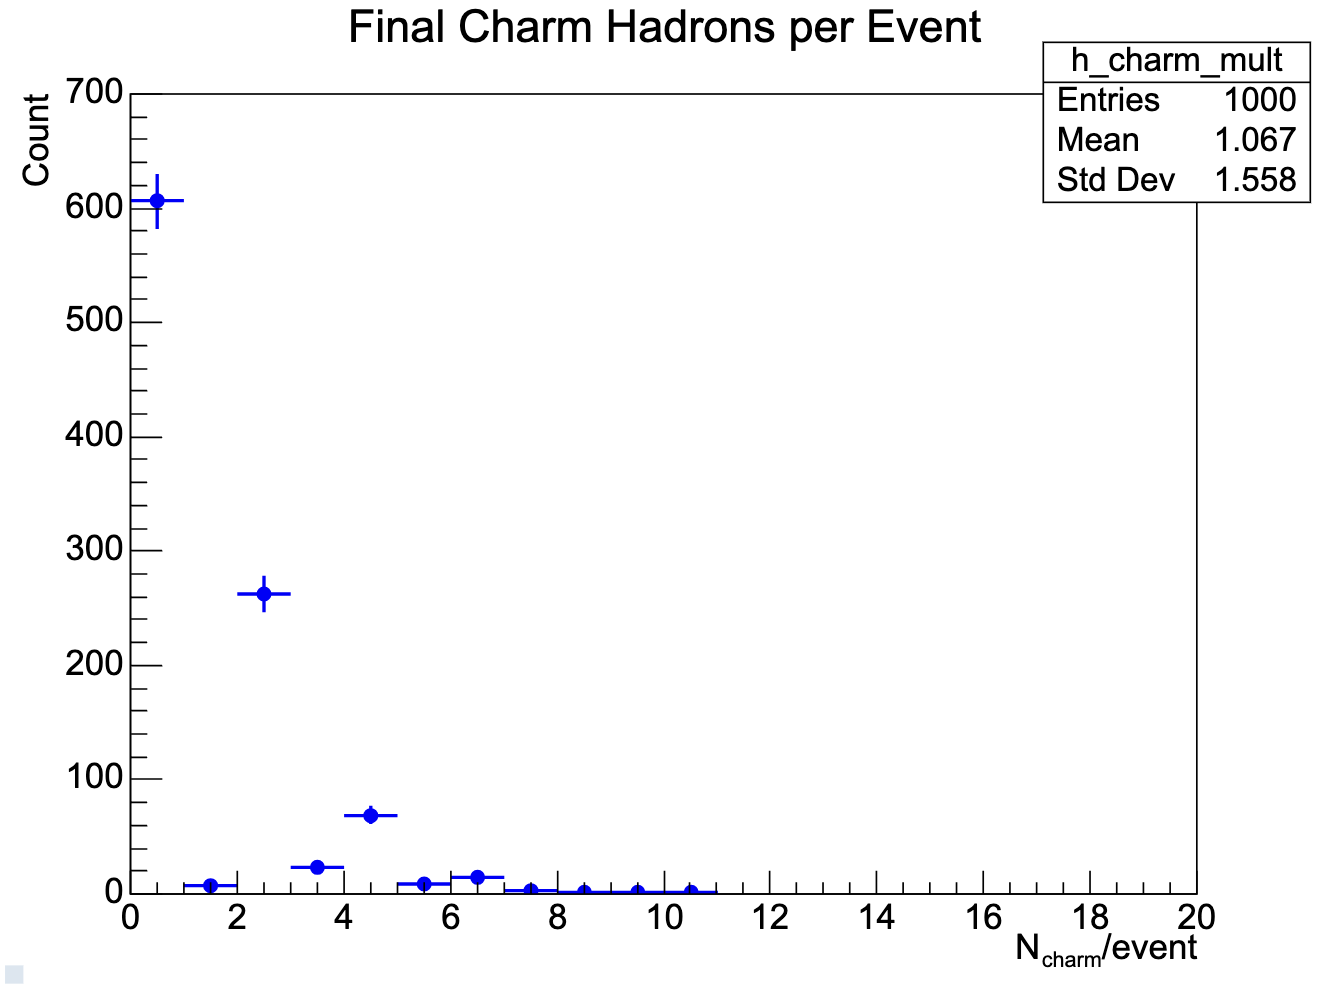
\includegraphics[width=0.8\linewidth]{Dstardecay.png}
    \caption{Charmed "final" hadron counts. Clear pair bias now. Still a few odd events which correlates to the rarity of flavor excitation}
    \label{fig:D* Decay}
\end{figure}
\end{frame}

\begin{frame}{Charm Counts Probability Distribution}

\begin{figure}
    \centering
    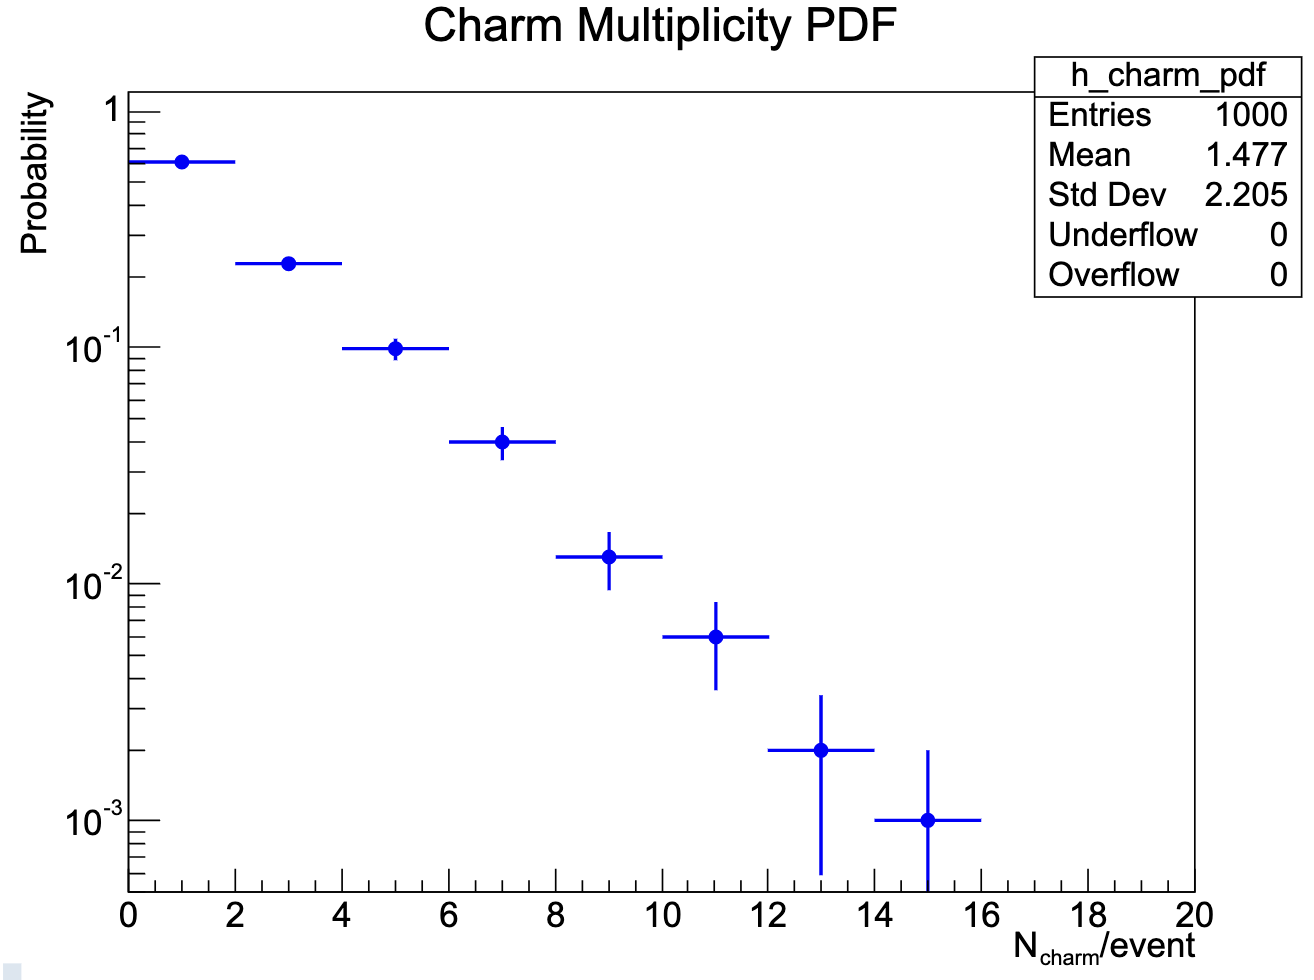
\includegraphics[width=0.6\linewidth]{charmPDF.png}
    \caption{Charm production counts with Bin Width of 2 }
    \label{fig:PDF}
\end{figure}
\begin{itemize}
    \item Integrating from 2 to inf yields $P(N_c\geq2) = 0.3880 \pm 0.0247$ 

    \item Note the exponential behavior
\end{itemize}
\end{frame}

\begin{frame}{Charm Quark Multiplicity}

\begin{figure}
    \centering
    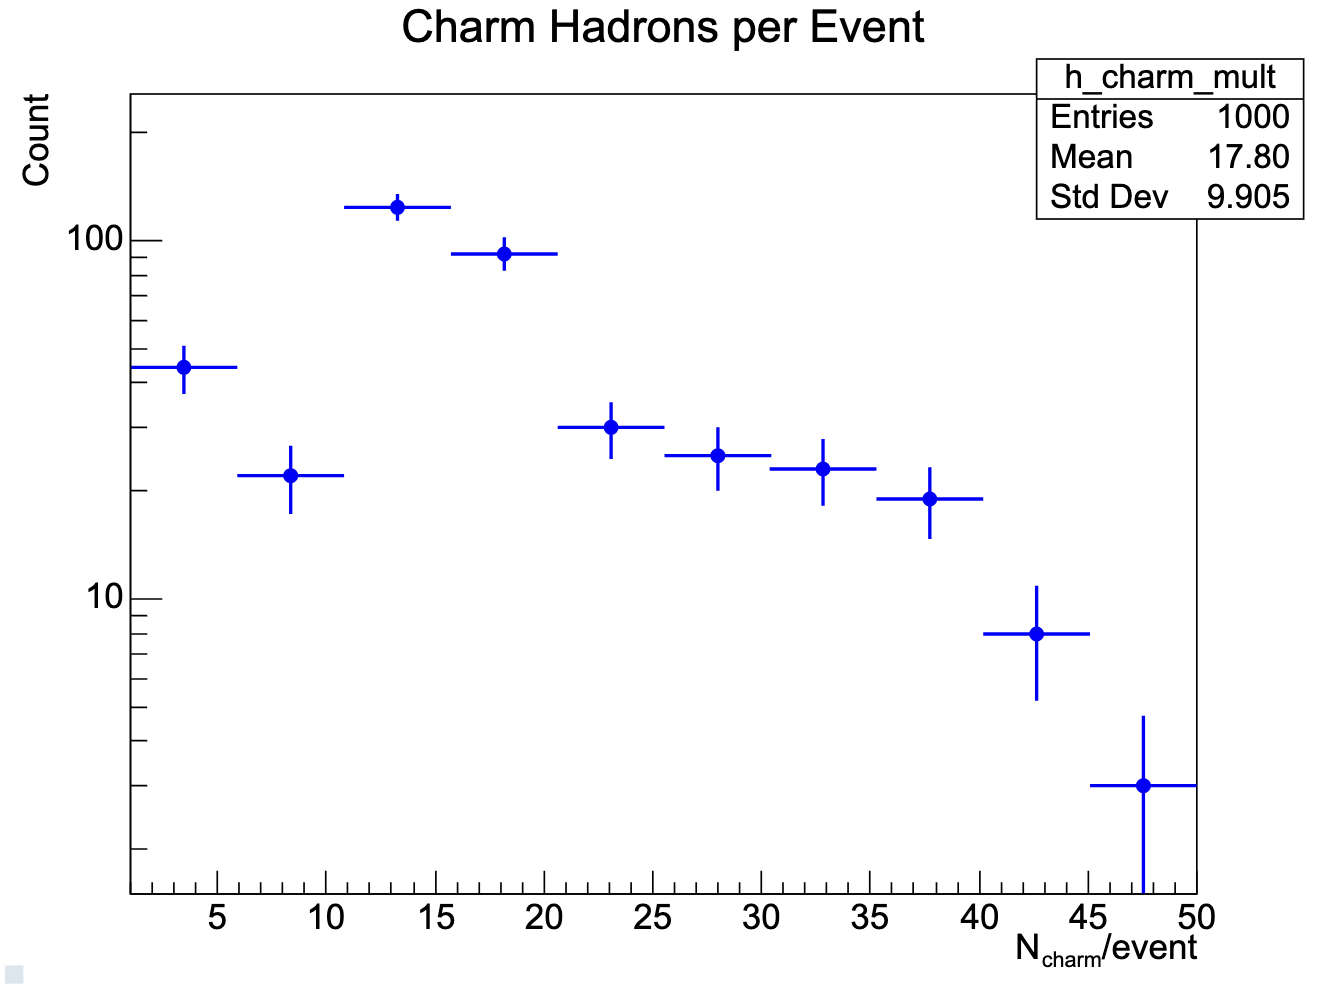
\includegraphics[width=0.7\linewidth]{quarkmult.png}
    \caption{I experimented by adding in the multiplicity of charm hadrons + charm quarks to the production histogram. \textbf{Note:} there are many charm quarks counted}
    \label{fig:quark mult}
\end{figure}
    
\end{frame}

\begin{frame}{Charm Quark Multiplicity}

There are many charm quarks counted. This is misleading though, because we are parsing through all particles through the decay chain. 

If we count a charmed hadron, we also counted all the vertexes previously with its charm quark. A similar pattern emerges due to jet fragmentation.

$\rightarrow$ Leads to massive double counting.
    
\end{frame}

%%%%
\section{Kinematic Correlations}

\begin{frame}{Overview}

\begin{itemize}
    \item When doing kinematic analysis, 1,000 events was not enough. The plots were too noisy, so I worked with 10,000 events. 
    \item We will conduct analysis on the "final" charm hadrons.
    \item I also did kinematic analysis only on events which contained \textit{only }two charm quarks, as we expect these to be correlated.

\vspace{1em}
We will look at $pT, y, \eta, \phi,$ and $\Delta\phi$ of the charmed hadrons
\end{itemize}

\end{frame}

\begin{frame}{Transverse momentum}
\begin{figure}
    \centering
    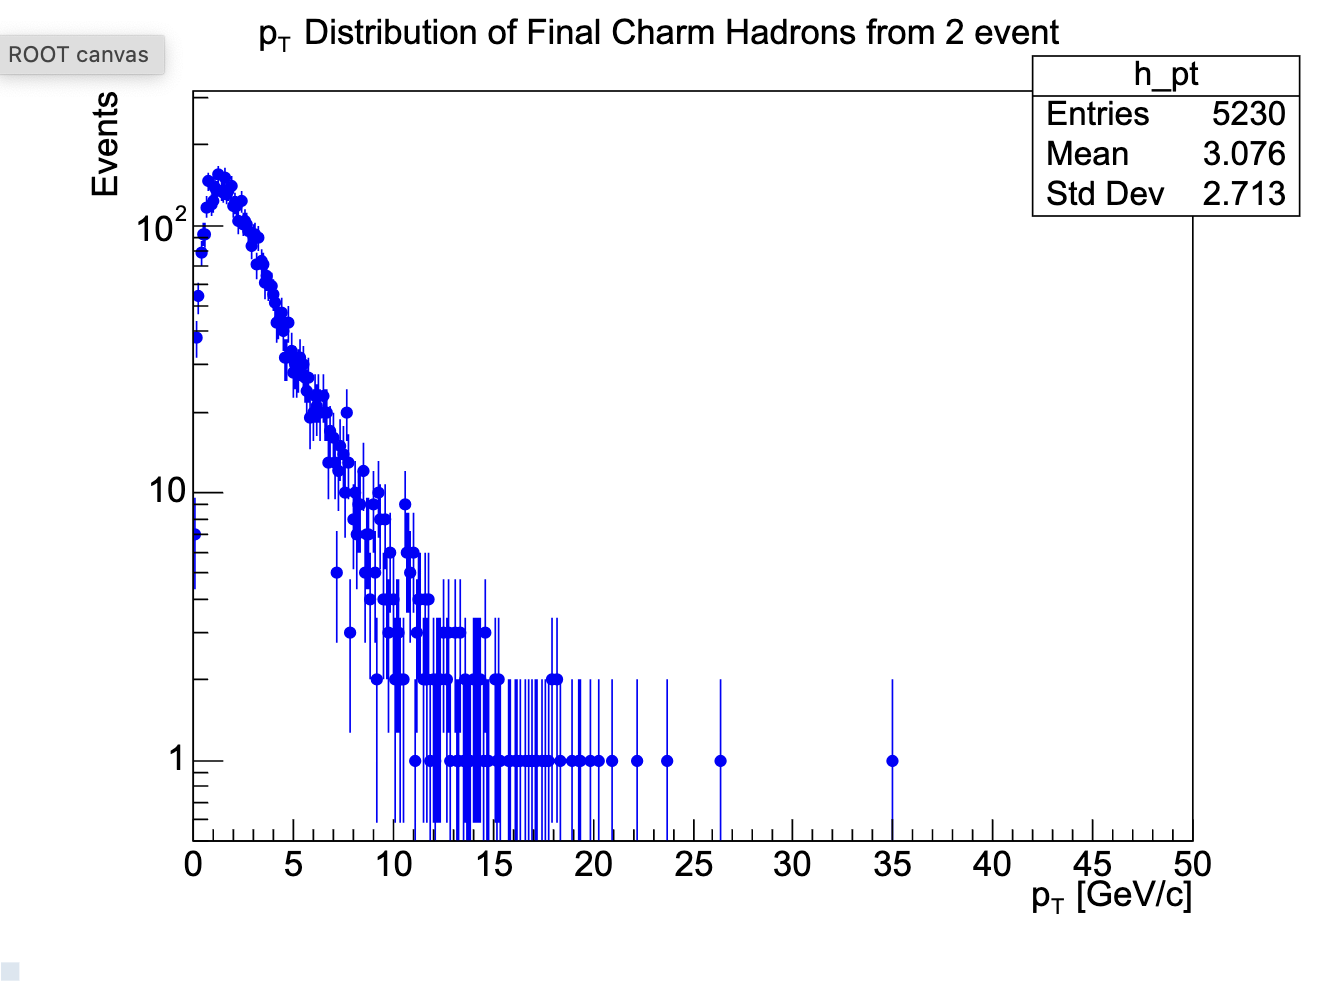
\includegraphics[width=0.8\linewidth]{transverse.png}
    \caption{The $pT$ distribution for charmed hadrons}
    \label{fig:transverse}
\end{figure}
\end{frame}

\begin{frame}{Transverse Momentum}

\begin{itemize}
    \item It is low near $pT=0$ GeV/c $\rightarrow$ Charm quarks are produced in hard QCD processes, where some momentum transfer is required, so it is kinematically supressed.
    \item There is a peak at \textasciitilde 2 GeV, indicating the usual range for charmed hadrons.
    \item The drop off after 2 GeV, especially with the log scale, indicates the rarity of higher pT charm hadrons.
\end{itemize}
\end{frame}

\begin{frame}{Rapidity and Pseudorapidity}
    \begin{figure}
        \centering
        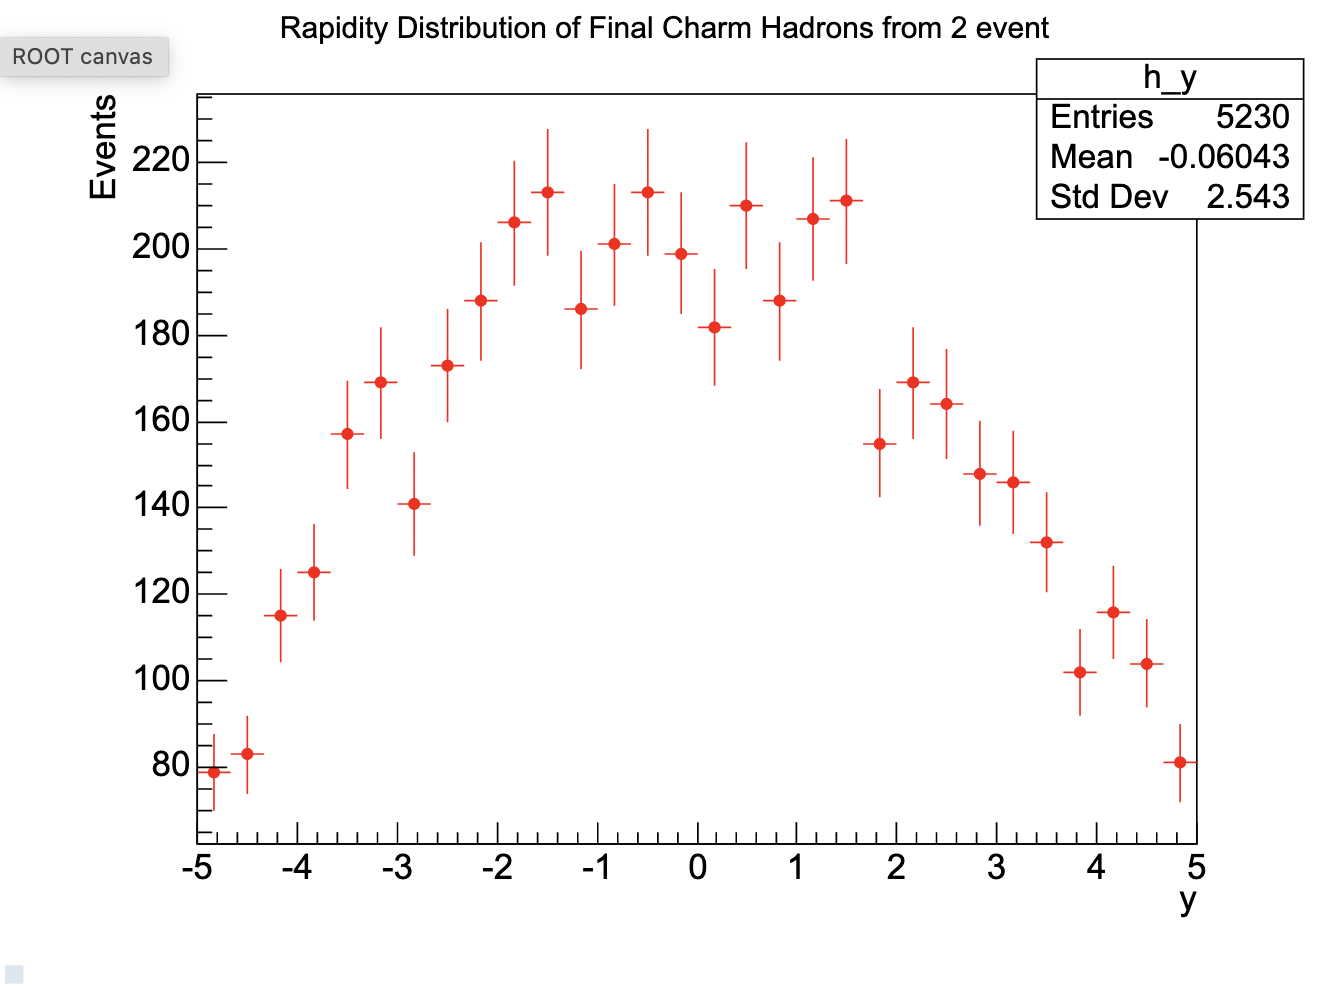
\includegraphics[width=0.8\linewidth]{rapidity.png}
        \caption{Rapidity distribution. \textbf{Note:} The peak at 0}
    \end{figure}
\end{frame}

\begin{frame}{Rapidity and Pseudorapidity}
    \begin{figure}
        \centering
        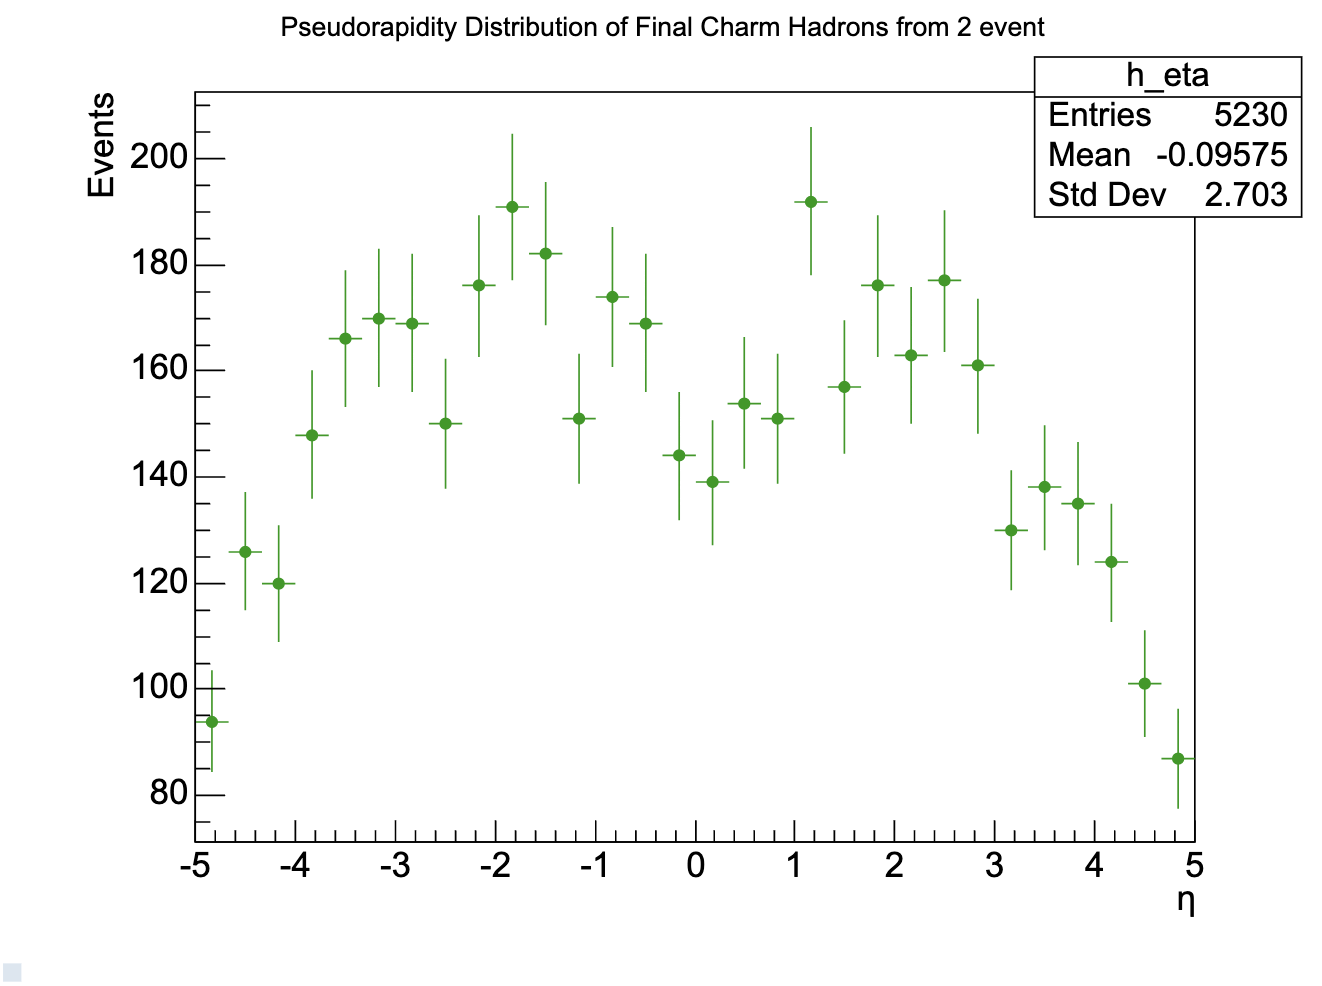
\includegraphics[width=0.8\linewidth]{eta.png}
        \caption{Pseudoapidity distribution. \textbf{Note:} The dip at 0}
    \end{figure}
\end{frame}

\begin{frame}{Rapidity and Pseudorapidity}
These distributions relate to the polar angle with respect to the beamline
    \begin{itemize}
        \item On average, the particles are centered around the pT plane with y = 0. (Polar angle of 90)
        \item Fewer particles are going in the direction of the beamline (very positive or negative values)
        \item There is a dip in $\eta$ at 0 due to the way it is calculated.
    \end{itemize}
\end{frame}

\begin{frame}{Phi}
\begin{figure}
    \centering
    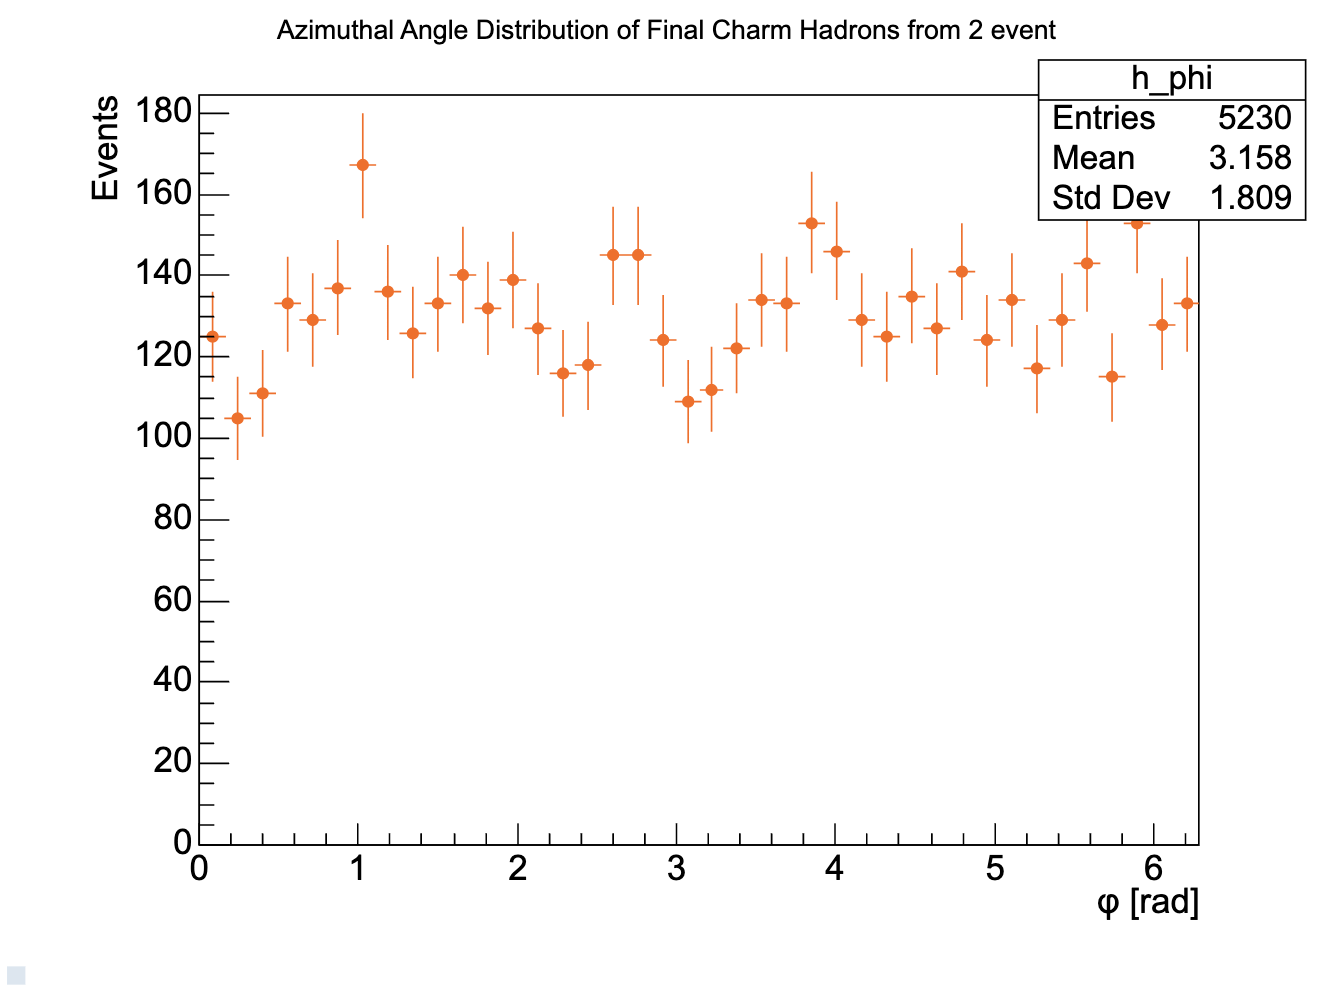
\includegraphics[width=0.7\linewidth]{phi.png}
    \caption{Phi distribution. \textbf{Note:} It is randomly spread}
\end{figure}

The random spread indicates that there is no bias towards a specific direction in the pT plane.
\end{frame}

\begin{frame}{Delta Phi: Hadrons}
\begin{figure}
    \centering
    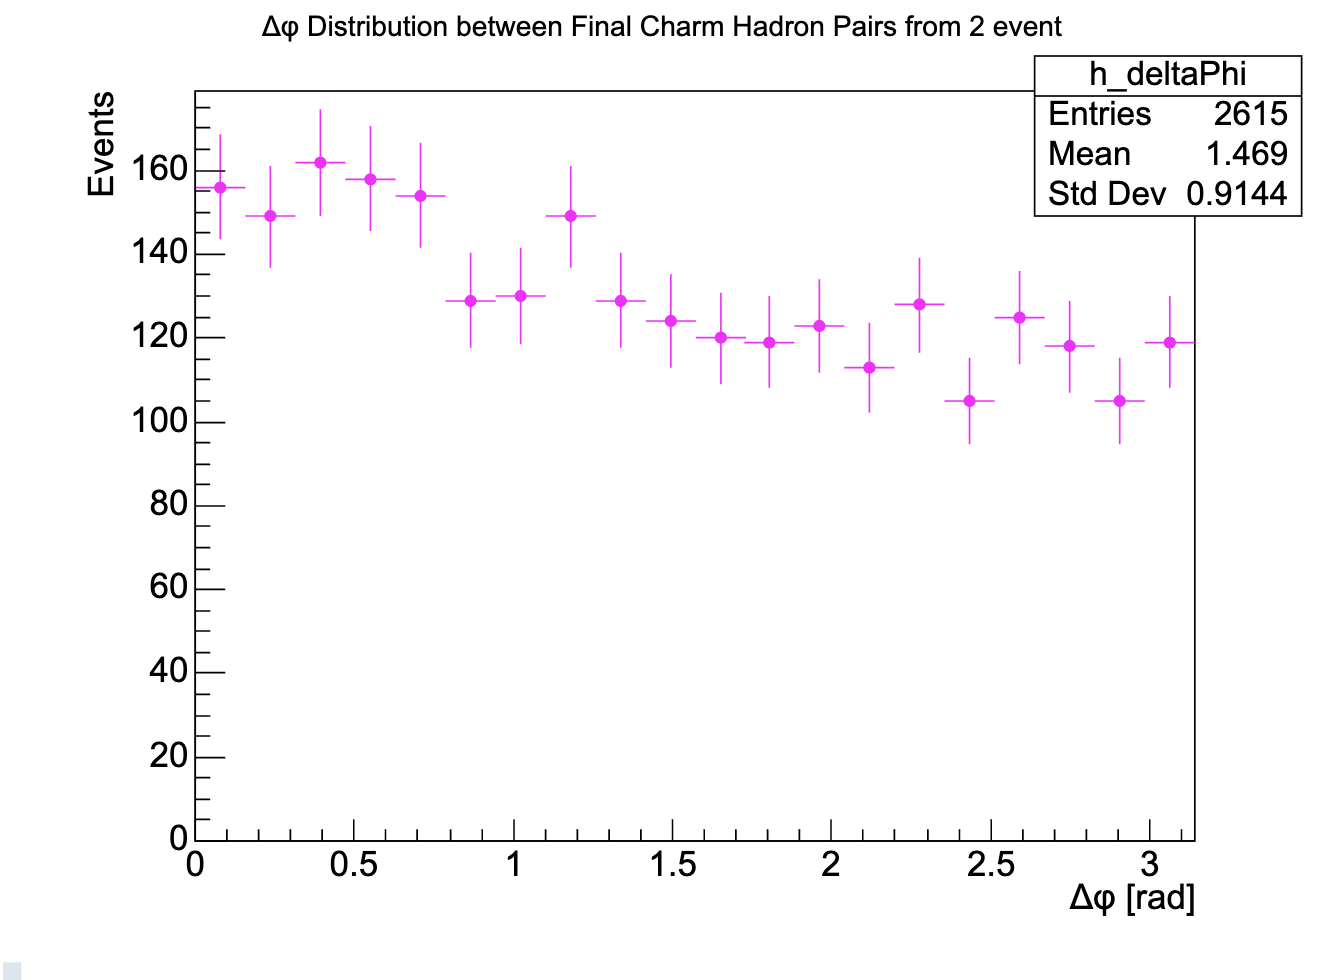
\includegraphics[width=0.6\linewidth]{dphi2.png}
    \caption{$\Delta\Phi$ distribution. \textbf{Note:} It is randomly spread}
\end{figure}

This is concerning - we expect there to be strong correlations, especially because we only picked events which have 2 charmed hadrons which should be correlated. We expect a peak at 0 and a broad peak on the away side.
\end{frame}

%%%%%%
\begin{frame}{Including all events}

I conducted the same analysis without filtering for 2 events. and got similar results for all the kinematics.
    
\end{frame}

\begin{frame}{Transverse momentum}
\begin{figure}
    \centering
    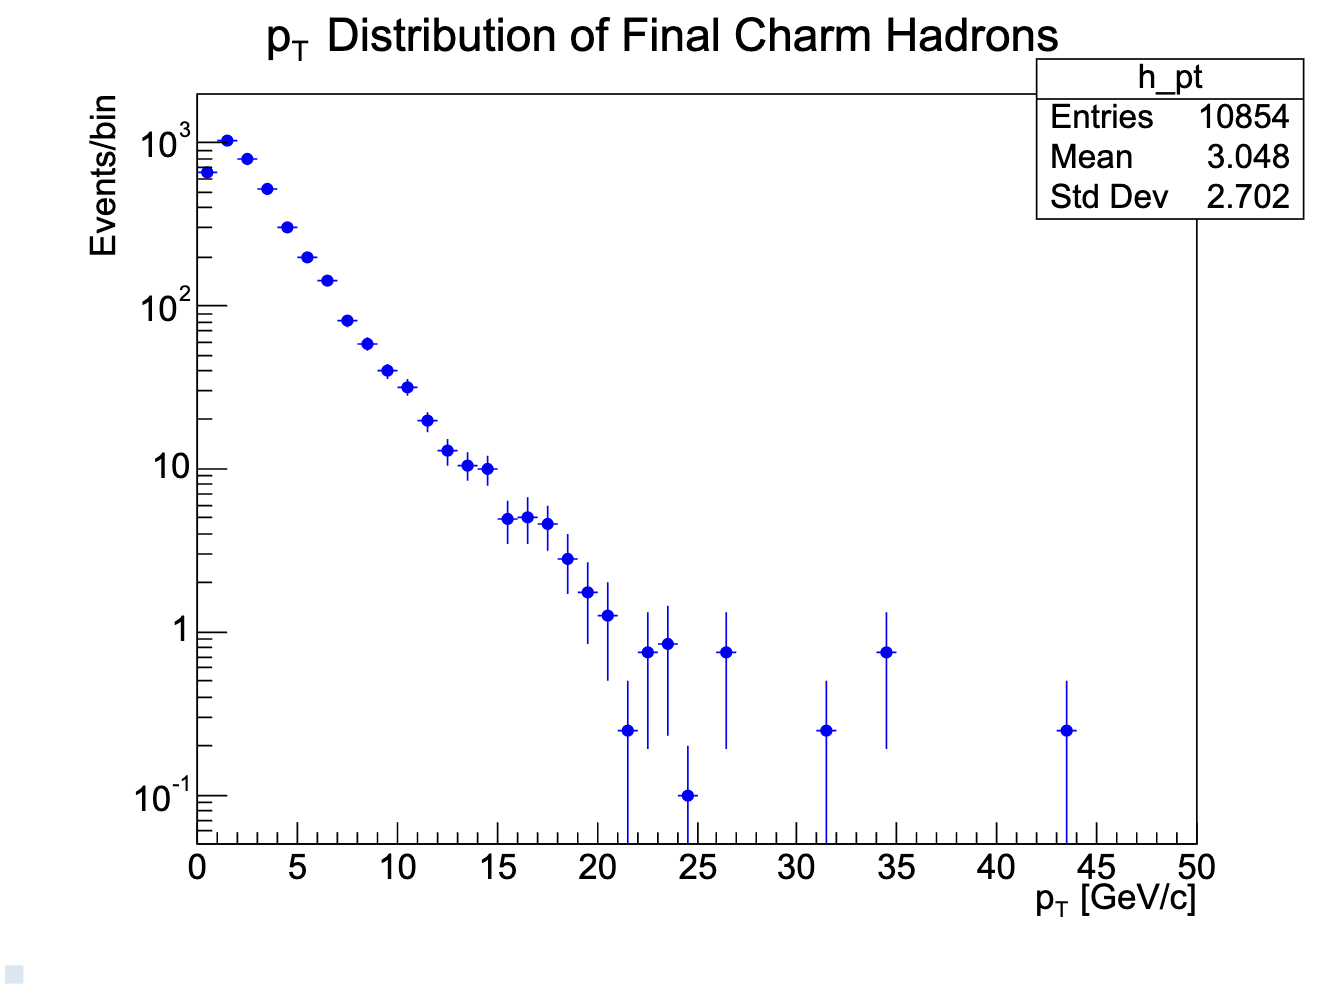
\includegraphics[width=0.8\linewidth]{pt all.png}
    \caption{The $pT$ distribution for charmed hadrons}
\end{figure}
\end{frame}

\begin{frame}{Rapidity and Pseudorapidity}
    \begin{figure}
        \centering
        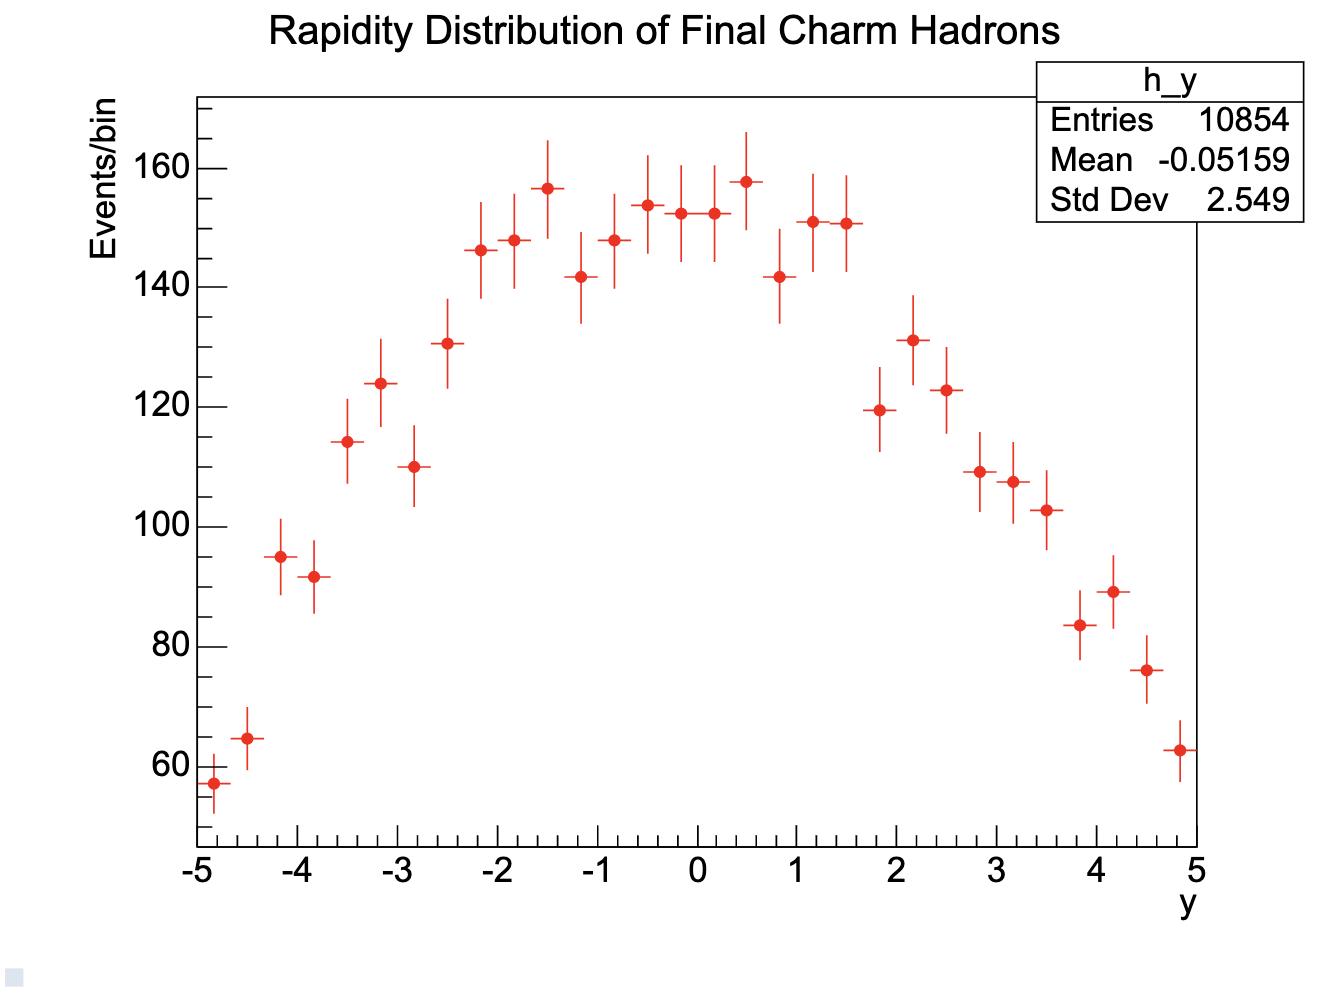
\includegraphics[width=0.8\linewidth]{y all.png}
        \caption{Rapidity distribution. \textbf{Note:} The peak at 0}
    \end{figure}
\end{frame}

\begin{frame}{Rapidity and Pseudorapidity}
    \begin{figure}
        \centering
        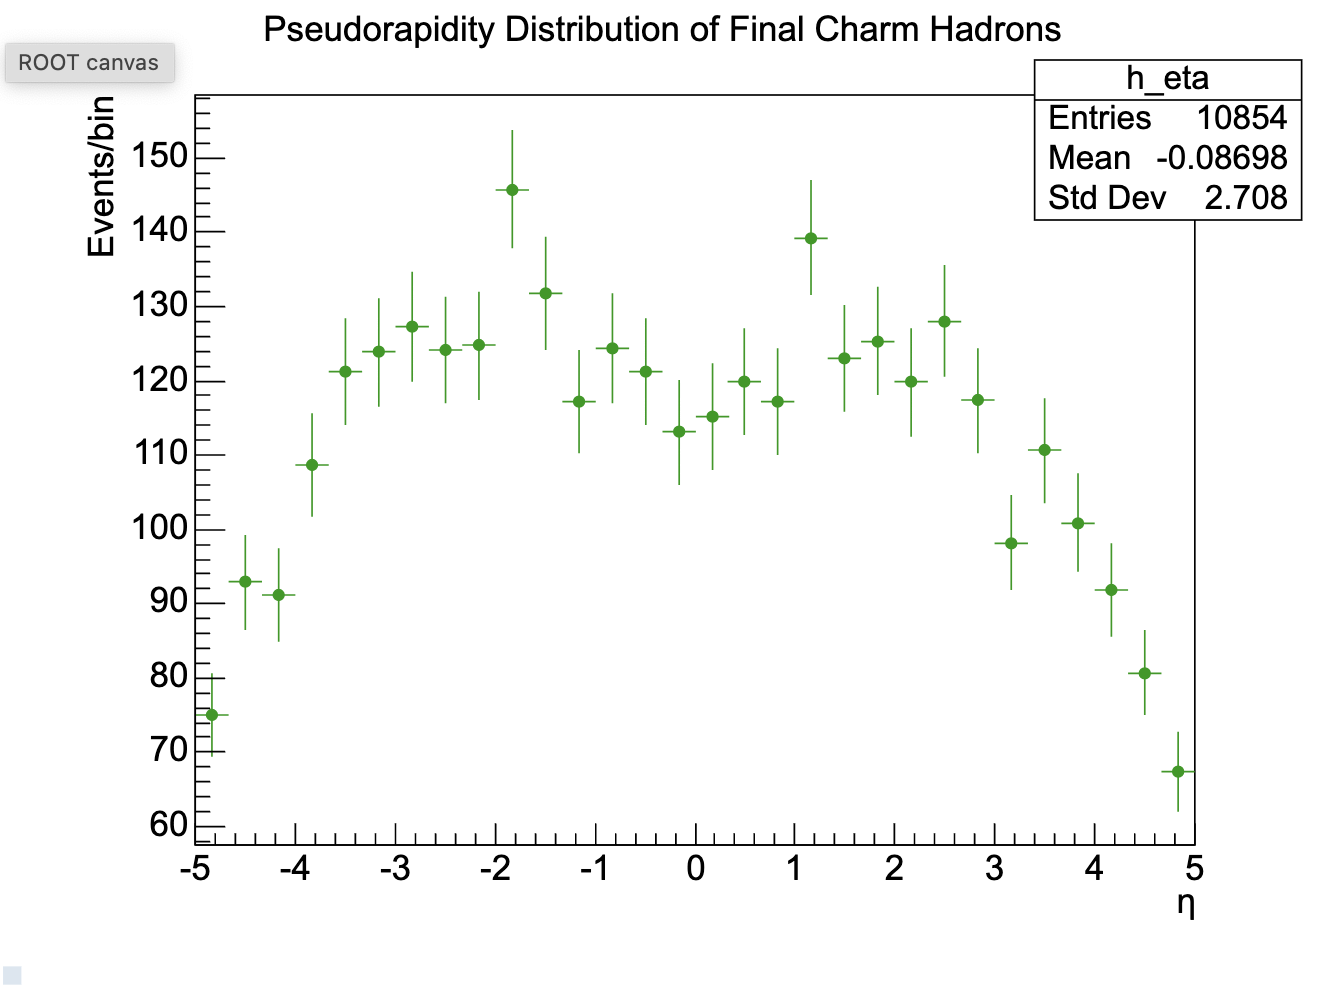
\includegraphics[width=0.8\linewidth]{eta all.png}
        \caption{Pseudoapidity distribution. \textbf{Note:} The dip at 0}
    \end{figure}
\end{frame}

\begin{frame}{Delta Phi: D0 Trigger}
\begin{figure}
    \centering
    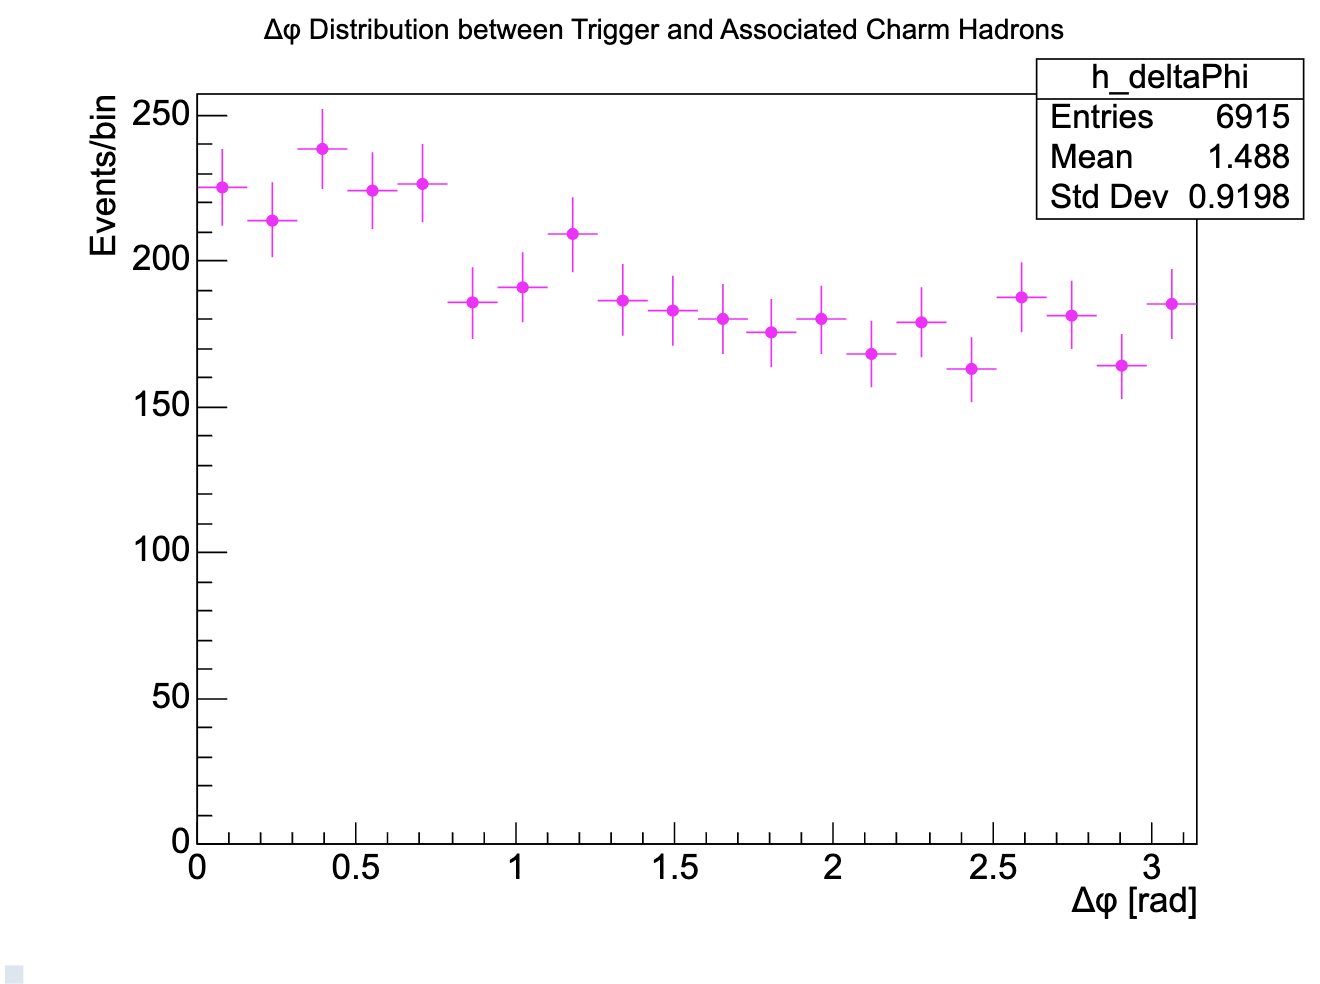
\includegraphics[width=0.6\linewidth]{phi trigger.png}
    \caption{$\Delta\Phi$ distribution. \textbf{Note:} Triggered on D0, with associated particles being all other charmed hadrons}
\end{figure}
We still see the same concerning behavior.
\end{frame}

\begin{frame}{Delta Phi: D0 Trigger with all other particles}
\begin{figure}
    \centering
    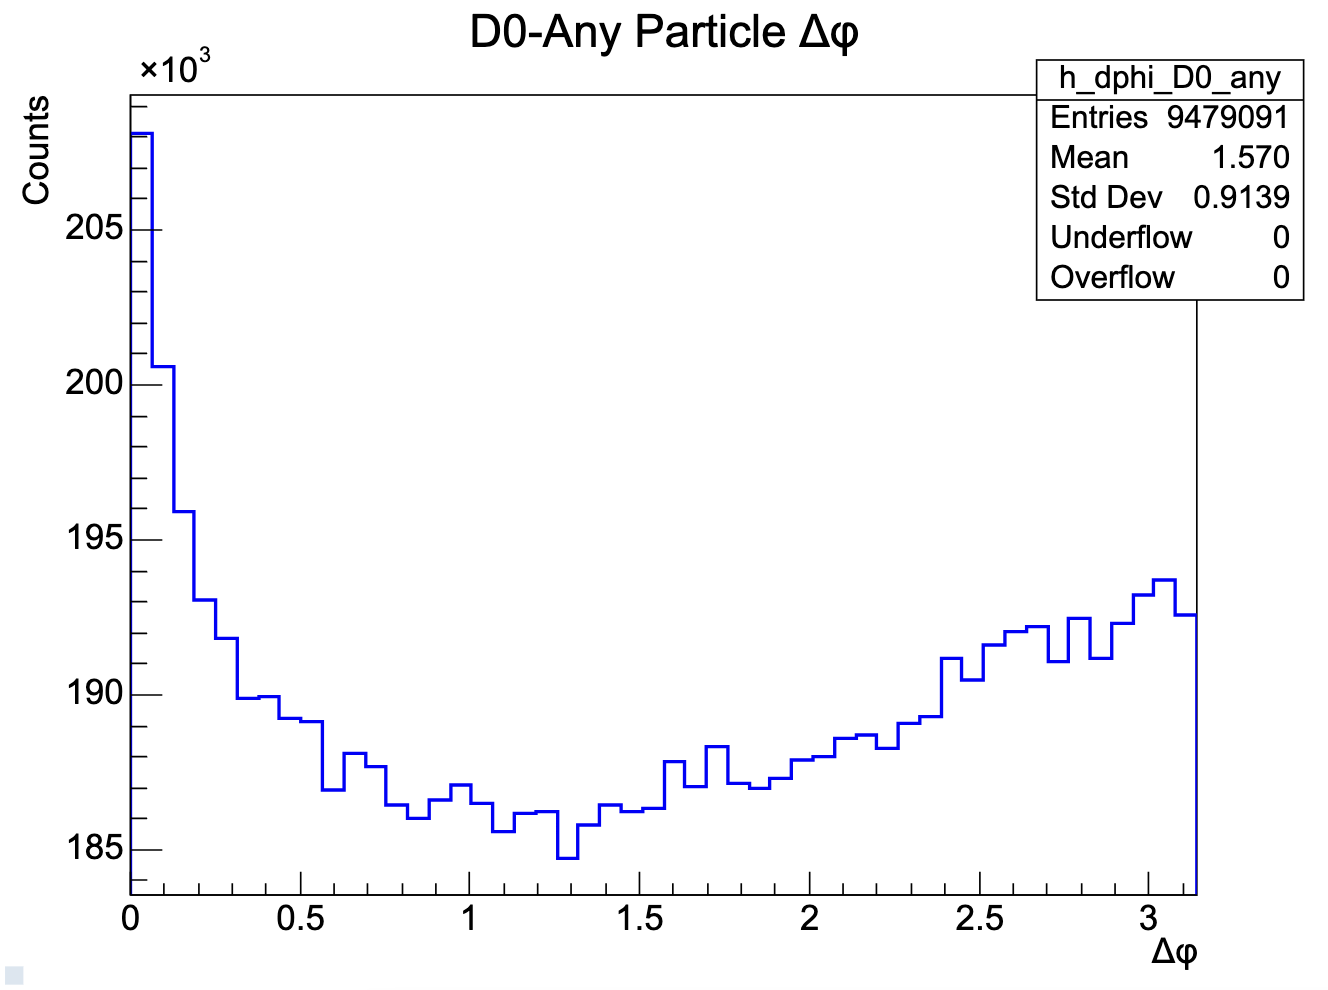
\includegraphics[width=0.6\linewidth]{dphi all.png}
    \caption{$\Delta\Phi$ distribution. \textbf{Note:} Triggered on D0, with associated particles being all other particles}
\end{figure}
This shows the correlation which we want - a peak at 0 and a broad peak away.
\end{frame}

\begin{frame}{Delta Phi: D0 Trigger with all other particles}
\textbf{Sharp peak at 0} $\rightarrow$ in gluon splitting, there is 1 gluon which splits into 2 charm quarks. These quarks are close to collinear, leading to front to front peak being sharp

\textbf{Broad peak at $\pi$} $\rightarrow$ in pair production, there is 2 gluons which become 2 charm quarks. These quarks are opposite in phi, leading to back to back correlations. Due to fragmentation and other interactions, the peak smears.
\end{frame}

\begin{frame}{2D Correlation Map}

\textbf{To revisualize the data, we can use a 2D heatmap and trigger on a D0.} (Trigger on D0 because it is produced the most)
    
\end{frame}

\begin{frame}{pT 2D}
\begin{figure}
    \centering
    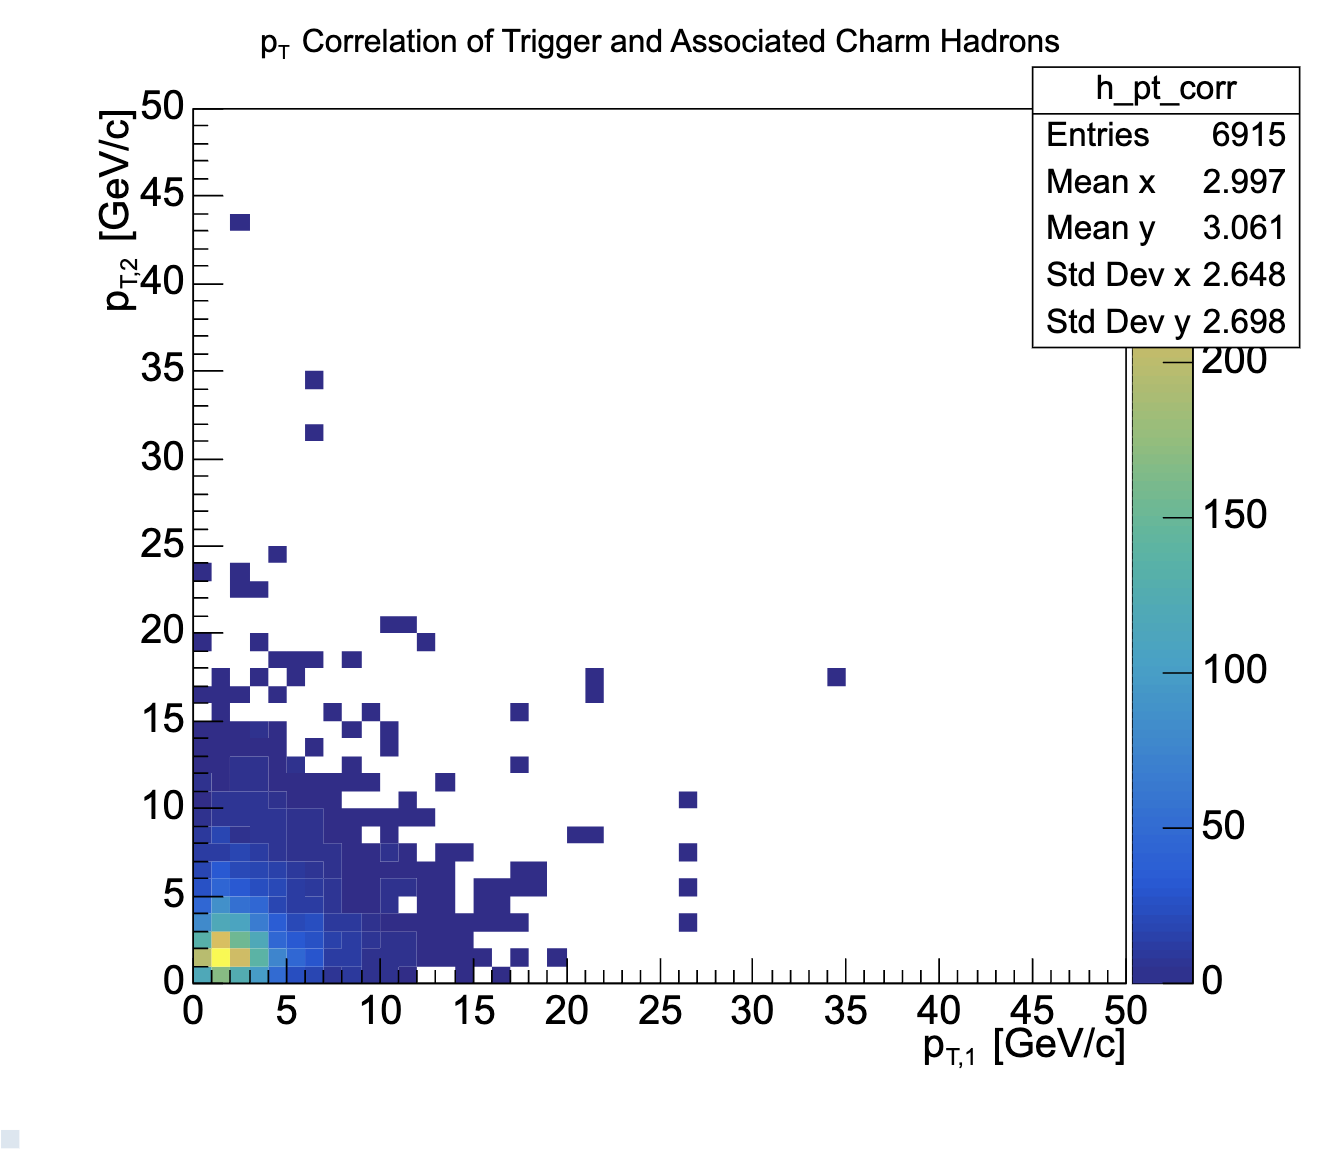
\includegraphics[width=0.8\linewidth]{2dpt.png}
    \caption{2D pT Correlation.}
\end{figure}
    
\end{frame}

\begin{frame}{y 2D}
\begin{figure}
    \centering
    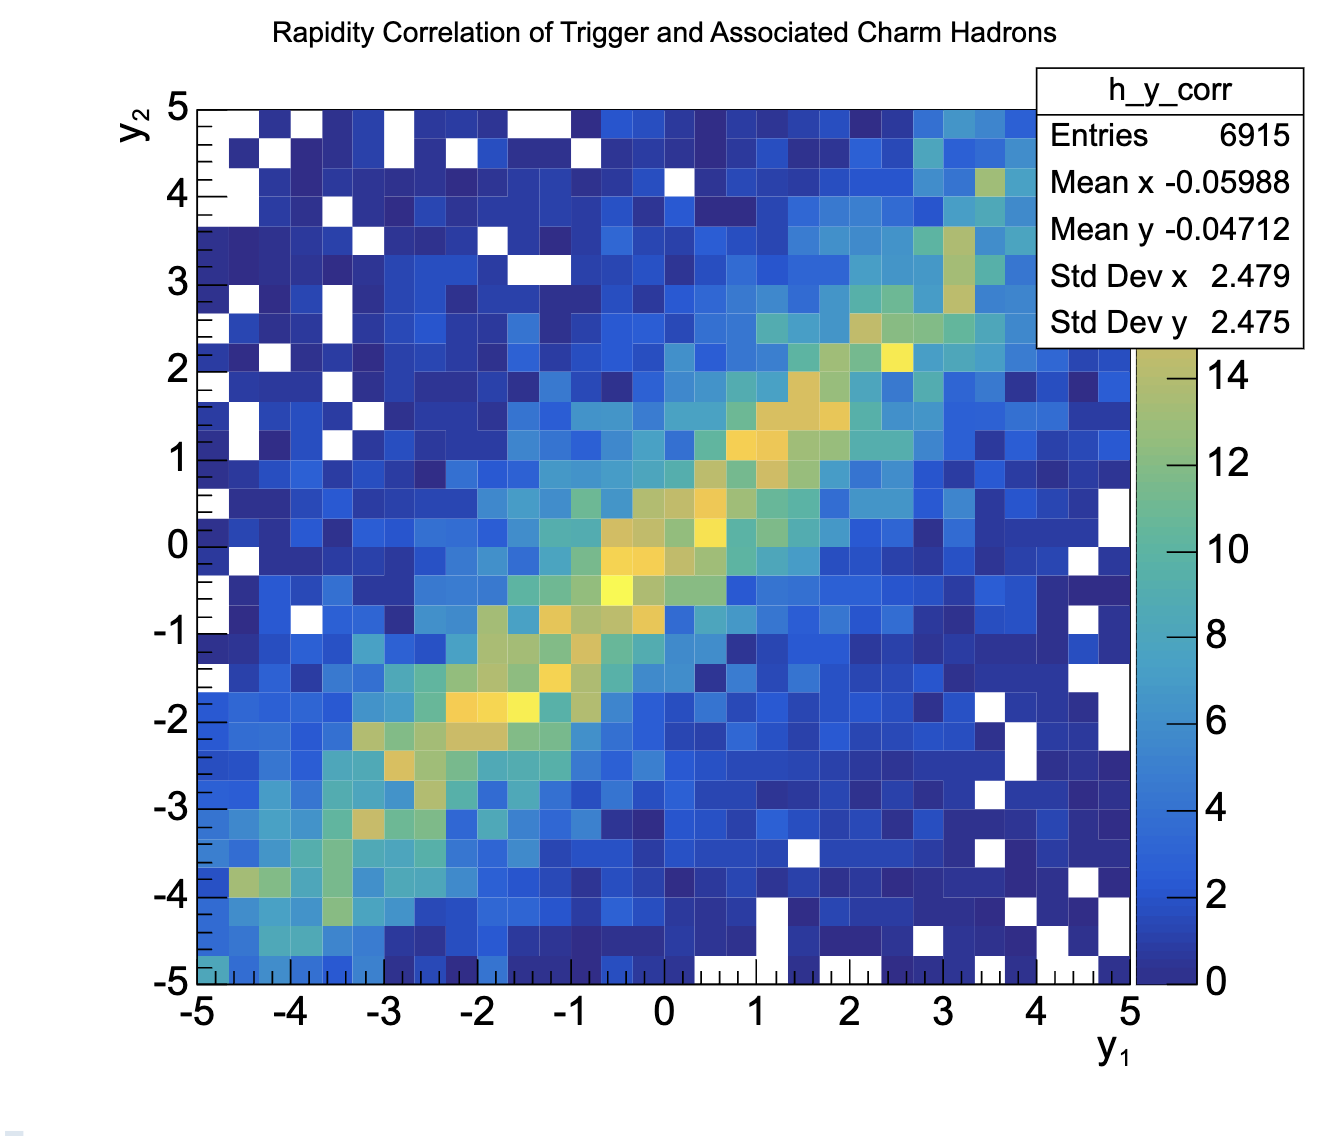
\includegraphics[width=0.8\linewidth]{2dy.png}
    \caption{2D y Correlation.}
\end{figure}
    
\end{frame}

\begin{frame}{$\eta$ 2D}
\begin{figure}
    \centering
    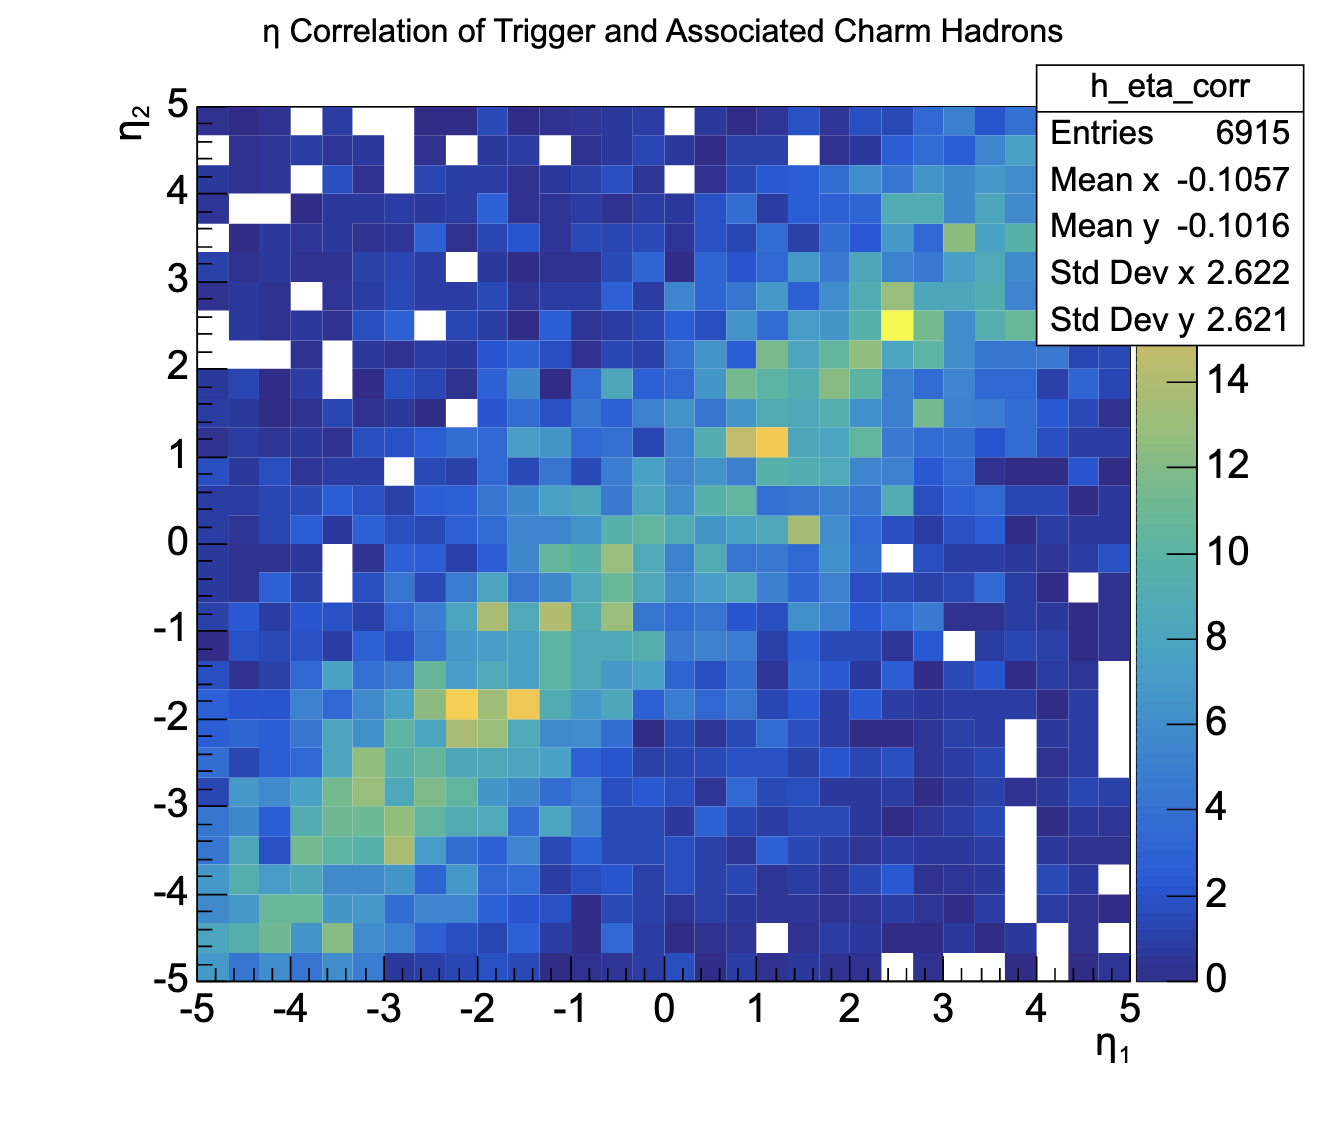
\includegraphics[width=0.8\linewidth]{2deta.png}
    \caption{2D $\eta$ Correlation.}
\end{figure}
    
\end{frame}

\begin{frame}{$\phi$ 2D}
\begin{figure}
    \centering
    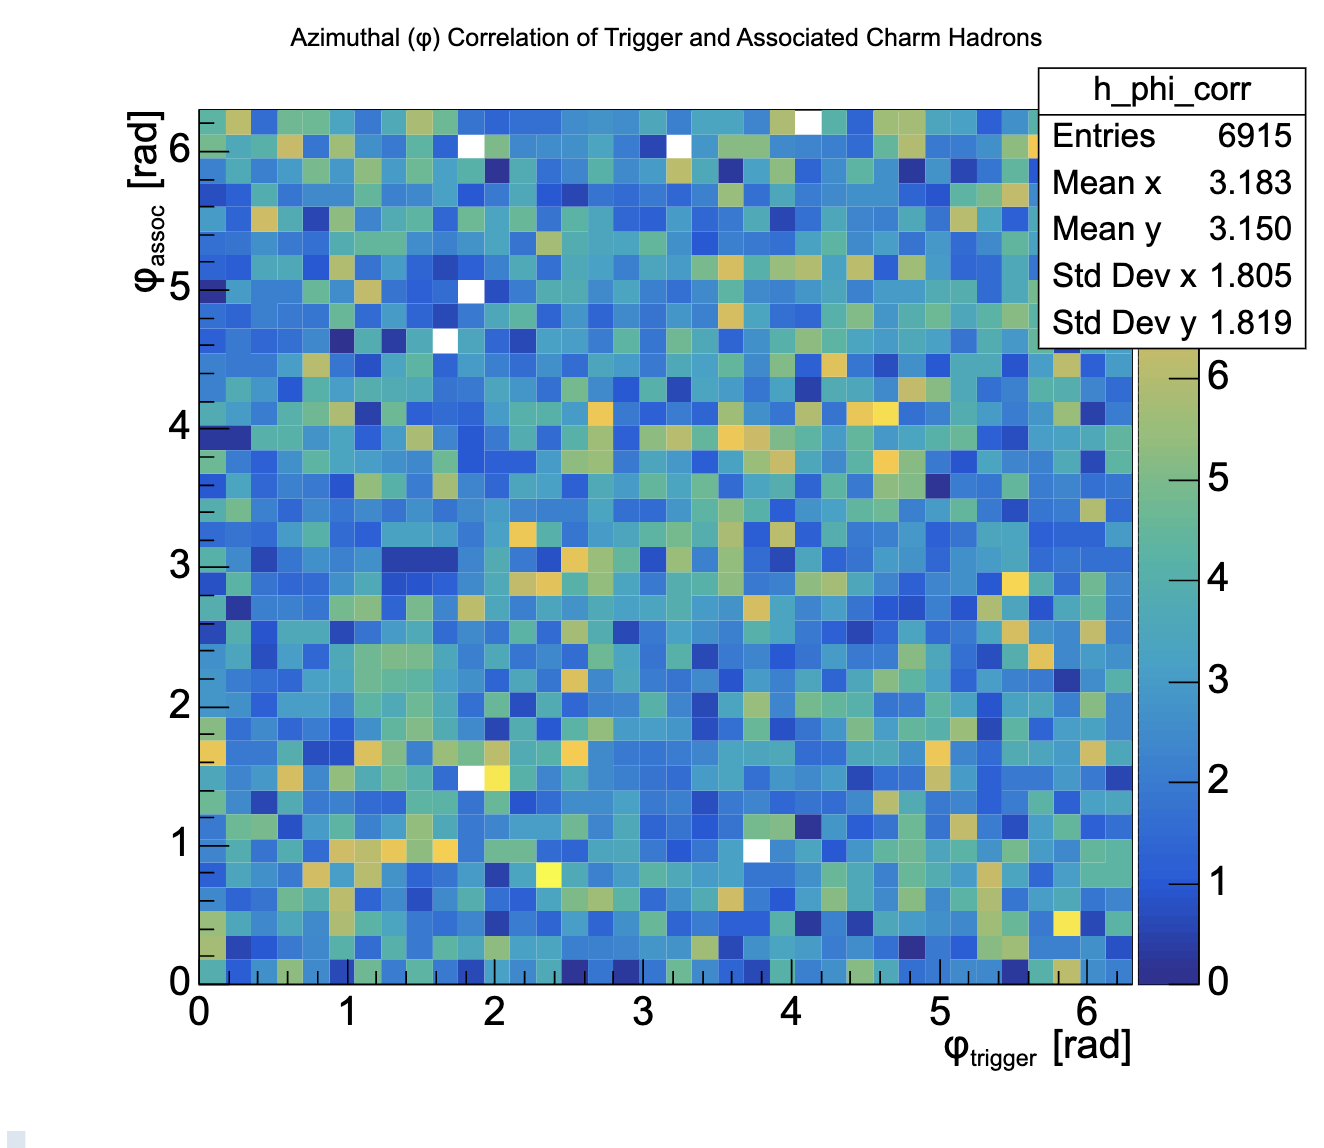
\includegraphics[width=0.6\linewidth]{2dphi.png}
    \caption{2D $\phi$ Correlation.}
\end{figure}
We can see the random behavior, similar to the $\Delta\Phi$ plot before. Why this occurs, I don't know yet. Cliffhanger!
\end{frame}


\section{Next Steps}

\begin{frame}{Next Steps}
\begin{enumerate}
    \item Probe the reason for the odd behavior for delta phi more. 
    \item Publish my repository to GitHub
    \item Return to write my thesis!
\end{enumerate}

    
\end{frame}

\section{Thank you for listening! Any questions?}


\end{document}